%\DeclarePairedDelimiter\abs{\lvert}{\rvert}
%\DeclarePairedDelimiter\norm{\lVert}{\rVert}

%\renewcommand\Re{\operatorname{Re}}
%\renewcommand\Im{\operatorname{Im}}

\renewcommand{\Re}{\mathcal{R}}
\renewcommand{\Im}{\mathcal{I}} 
%
\chapter{Background}
\label{ch:background}
%
Ocean surface waves are generated by different kinds of forces, such as 
storms, earthquakes, the gravity of sun and moon, but with~\emph{wind} being
the most prominent one. Each of these forces influences one or more frequency
bands of the electromagnetic wave spectrum. The combination of said frequency
bands constitutes the spectrum of ocean waves.
%
\begin{table}[h]
\begin{tabularx}{\textwidth}{X | X X | X X }
 %\hline
  \cline{2-5}
  & \multicolumn{2}{c}{Period Band Range (\si{\second})} \vline & \multicolumn{2}{c}{Frequency Band Range (\si{\hertz})} \\
  \hline
  Wave Type & Start & End & Start & End \\
 \hline
  Capillary    & $0$                & $1\times10^{-1}$   & $\infty$            & $1\times10^1$ \\
  Ultragravity & $1\times10^{-1}$   & $1\times10^{0}$    & $1\times10^1$       & $1\times10^0$ \\
  Gravity      & $1\times10^{0}$    & $3\times10^{1}$    & $1\times10^0$       & $3.33\times10^{-2}$ \\
  Infragravity & $3\times10^{1}$    & $3\times10^{2}$    & $3.33\times10^{-2}$ & $3.33\times10^{-3}$ \\
  Long Period  & $3\times10^{2}$    & $4.32\times10^{4}$ & $3.33\times10^{-3}$ & $2.32\times10^{-5}$ \\
  Tidal        & $4.32\times10^{4}$ & $8.64\times10^{4}$ & $2.32\times10^{-5}$ & $1.16\times10^{-5}$ \\
  Transtidal   & $8.64\times10^{4}$ & $\infty$           & $1.16\times10^{-5}$ & $0$
\end{tabularx}
\caption{A classification of ocean surface waves by period and frequency.}
\label{tab:ocean_wave_period}
\end{table}
%

Table~\ref{tab:ocean_wave_period} gives a compact overview of different kinds 
of ocean surface waves classified by period band as well as the corresponding 
frequency band. The shortest period waves are the~\emph{capillary waves}, with 
periods less than \SI{0.1}{\second}. These are the first waves which one is able to notice 
when the wind starts to blow on the ocean surface, they appear like a fine
structure of small ripples of nearly capillary dimension.
% That is, capillary waves are largely responsible for what might be called the 
% inherent roughness of the surface, therefore they determine the effectiveness 
% with which the wind is able to grip the water.
Next are the~\emph{ultragravity waves} with periods ranging from \SI{0.1}{\second}
to \SI{1}{\second}. The ordinary~\emph{gravity waves} observed at sea have periods
varying from \SI{1}{\second} to \SI{30}{\second} and are composed of two types
of waves, namely~\emph{sea waves} and~\emph{swell}.
Sea waves are gravity waves directly generated and affected by local winds,
and after the wind ceases to blow they are called swell.
More generally, swell
consists of wind generated gravity waves that are not significantly affected
by the local wind, therefore they have  been generated elsewhere or at some
time in the past.
Beyond the ordinary 
gravity waves there are~\emph{infragravity waves}, with periods between \SI{30}{\second} 
and \SI{5}{\minute}. Then there are the~\emph{long period waves} with periods in the 
range \SI{5}{\minute} to \SI{12}{\hour}. Their representatives in the sea are tsunamis 
and storm surges. The~\emph{ordinary tidal waves} represent the astronomical 
tides with fixed wave periods of about \SI{12}{\hour} and \SI{24}{\hour}. At the end of the 
spectrum there are the~\emph{transtidal waves} with periods greater than 
\SI{24}{\hour}. These include the longer period components of astronomical tides.
%
\begin{figure}
  \centering
  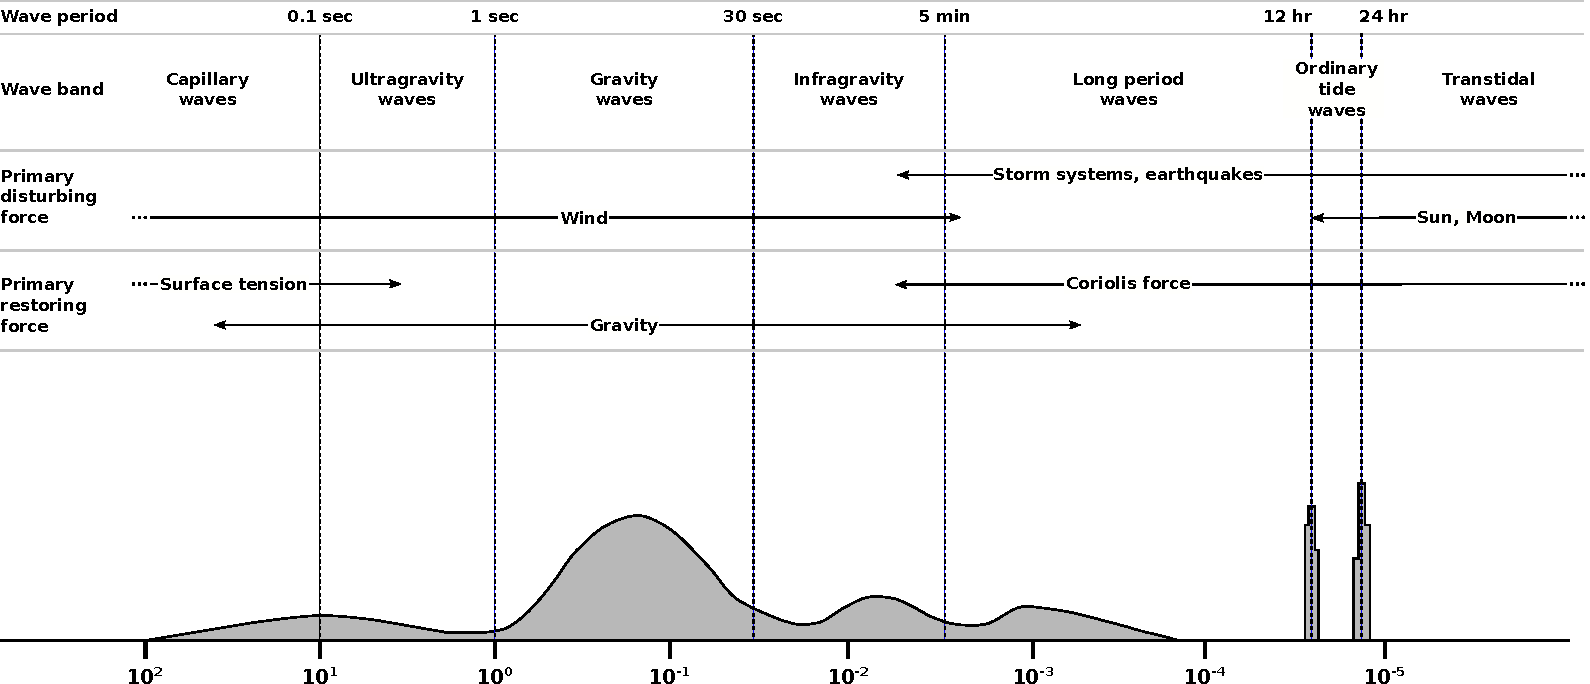
\includegraphics[width=\textwidth]{figures/SurfaceWavesEnergy}
  \caption{A tentative overview of which forces influence which wave 
  frequency band, as well as the relative amount of energy
  each wave frequency band contains. Source: \citet{article:munkorigin}}
  \label{fig:surface_waves_energy}
\end{figure}
%

Ocean surface waves are also classified by their major governing forces.
One, the disturbing force which causes the actual water displacement,
and second, the restoring force which brings the water back to its position
at rest. Winds are responsible for the generation of capillary waves,
ultragravity waves, gravity waves and infragravity waves, whereas long
period waves like tsunamis are generated by storms and earthquakes.
The ordinary tides are caused by the gravitational pull of sun
and moon, transtidal waves on the other hand by storms, sun and moon.
As soon as the water has been displaced, the force to bring capillary
waves back to their position at rest is exerted by surface tension.
Ultragravity waves, gravity waves and infragravity waves have gravity
as their major restoring force. Gravity together with coriolis act
as the restoring force for long period waves, ordinary tidal waves and
transtidal waves.
% One, the disturbing force which causes the actual water displacement,
% such as wind, storms, earthquakes, and the gravity of sun and moon.
% Second, the restoring force which brings the water back to its position at
% rest, such as surface tension, gravity, and coriolis.
% Winds are responsible for the generation of capillary waves,
% ultragravity waves, gravity waves and infragravity waves. Storms and
% earthquakes generate long period waves like tsunamis, whereas the
% gravitational pull of sun and moon is responsible for ordinary tidal
% waves. Moreover, storms, sun and moon are the source of trans-tidal
% waves.
Figure~\ref{fig:surface_waves_energy} pictures the entire spectrum
of ocean surface waves and the forces responsible for various portions
of the spectrum. As one can see, gravity is the main restoring force,
therefore ocean surface waves are classified as~\emph{surface gravity waves}.
Most of the energy of the spectrum is contained in two of the period
ranges: the ordinary gravity waves, and the ordinary tidal waves.
% These are the types of waves humans actually have in mind when they
% think of the ocean, as they are not only easy to observe with the
% naked eye, but have also affected humankind since the dawn of history.
Ordinary tidal waves, infragravity waves, long period waves, as well as
transtidal waves do not contribute significantly to the actual optical
appearance of the ocean in deep water, therefore we may omit them.
The remaining types of waves have wind as the common disturbing force
and are therefore grouped under the term \emph{wind generated waves},
or in short, \emph{wind waves}. Wind waves still contain large part of
the energy of the spectrum, and range from ripples with less than a
centimeter in height to huge waves more than thirty meters high.
% Such a variety of waves is sufficient to reproduce believable ocean
% surfaces under diverse conditions.
% Ocean surface waves generated by wind
% blowing over an area of fluid surface are called
% \emph{wind generated waves}, or in short,~\emph{wind waves}.

% Wind blowing over a vast stretch of the air-sea interface is the main
% force to generate waves on the ocean surface, this kind of waves is
% called~\emph{wind generated waves}, or in short,~\emph{wind waves}.

% and range from ripples with less than a centimeter in height to huge waves more
% than thirty meters high.


% Given the above classification, the ocean surface waves with the shortest period are the~\emph{capillary waves}. These are the first waves which one is able to notice when the wind starts to blow on the ocean surface. Capillary waves appear like a fine structure of small ripples of nearly capillary dimension, and
% as such they determine largely the optical effects of the surface. Moreover, they play an important role in the context of energy transfer from the wind to the water. That is, capillary waves are largely responsible
% for what might be called the inherent roughness of the surface, therefore they determine the effectiveness
% with which the wind is able to "'grip"' the water. Capillary waves are affected to a larger extent by surface
% tension than by gravity.
% 
% Next are \emph{gravity waves}, where the short ones are called \emph{ultra-gravity waves}, and the very long ones are called \emph{infra-gravity waves}.

% Because ocean surface waves are generated and propagate at the interface between the atmosphere
% and the ocean, where the restoring force of gravity is in effect, they are classified as~\emph{surface gravity waves}.
% Moreover, since wind blowing over a vast stretch of the air-sea interface is the main force to generate waves on
% the ocean surface, this kind of waves is called~\emph{wind generated waves},
% or in short,~\emph{wind waves}. Wind waves on the ocean surface represent
% gravity waves, while e.g. tsunamis and ocean tides do not.\\
% 
% The process behind surface gravity waves is a simple one - the moment a fluid element at the interface is displaced, gravity
% will try to restore it to equilibrium which results in oscillation of said fluid element. We mentioned before
% that wind is the most prominent force causing displacement on the water surface. As it blows, it causes pressure and friction
% forces which perturb the water surface's equilibrium. Therefore, the combination of wind transferring energy from the air
% to the water and gravitational acceleration cause the formation of waves on the water surface.\\
% 
In order to be able to model the surface of such an intricate fluid system as the ocean, one has to reduce complexity.
Research fields such as ocean engineering or coastal engineering employ the~\emph{Airy wave theory}~\citep{book:airy1845tides}
to model the properties of the sea. Airy wave theory, also known as~\emph{linear wave theory}, describes the propagation of
gravity waves on the surface of a homogeneous fluid with a set of~\emph{linear} equations. These equations give
a decent approximation of the wave dynamics and kinematics with enough accuracy to model the state of the sea over a
limited amount of time.

The remainder of this chapter is organized as follows:
Section~\ref{sec:linear_theory_ocean_waves} gives an introduction to linear wave theory
and its capability to model the ocean surface. Section~\ref{sec:random_sea}
presents the wave spectrum concept, whereas Section~\ref{sec:random_sea_discretisation}
outlines the steps necessary to synthesize an ocean surface based on
a wave spectrum.
Last, Section~\ref{sec:wave_spectra} discusses the wave spectra which we
implemented as part of this work.
% Last, Section~\ref{sec:wave_spectra} discusses various
% wave spectra obtained from oceanographic research, and one wave spectrum
% introduced in computer graphics literature.

\section{Linear Theory of Ocean Surface Waves}
\label{sec:linear_theory_ocean_waves}
Linear wave theory makes a set of assumptions about the properties of the fluid, such as its viscosity,
compressibility and curl. Because fluid dynamics, associated fluid properties, and the derivation
of the linear wave theory go beyond the scope of this thesis, we will refer the interested reader
to \citet{book:airy1845tides}, \citet{book:batchelor2000introduction}
and \citet{book:kinsman2002wind}.
\emph{But} we will mention two core assumptions of linear wave theory which are easy to picture:
\begin{itemize}
 \item The water body has a uniform mean depth.
 \item The wave amplitudes are small in relation to the size of the water body.
\end{itemize}
Suppose we observe an idealized ocean in which exactly one sine wave is travelling constantly.
The parameters defining the sine wave - amplitude, frequency, length and direction - are all fixed.
To simplify the mathematics we assume a two-dimensional ocean, with one
dimension representing the wave's direction of travel and the  other the wave's
vertical displacement. With these assumptions we can describe surface elevation
as a sinusoid:
%
\begin{equation}
\label{eq:sinusoid}
 \eta(x, t) = A\cos(kx - \omega t)
\end{equation}
with
\begin{align*}
\label{eq:sinusoid_parameters}
 k &= \frac{2\pi}{\lambda} & \omega &= 2\pi f & f &= \frac{1}{T}
\end{align*}
%
where $A$ is the amplitude, $k$ is called the~\emph{\wavenumber},~$x$ is the horizontal position,
$\omega$ is the~\emph{wave frequency} in radians per second,~$t$ represents the time,
$\lambda$ is the~\emph{\wavelength},~$f$ is the~\emph{wave frequency} in Hertz (\si{\hertz}) and~$T$
is the wave period in seconds. According to Airy wave theory, \wavenumber $k$
and angular frequency $\omega$ are not independent parameters, but are coupled
by the \emph{dispersion relation}. We will elaborate on the dispersion relation
at a later point, though.
% \begin{figure}
% 	\centering
% 	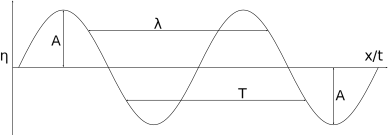
\includegraphics[width=\textwidth]{figures/sinusoid}
% 	\caption{An example of a sinusoidal wave.}
% 	\label{fig:sinusoid}
% \end{figure}
%
% \begin{figure}
% \begin{tikzpicture}
% \begin{axis}[domain=0:4*pi]
%     \addplot {sin(deg(x))}; 
%     \end{axis}
% \end{tikzpicture}
% \end{figure}
\begin{figure}
\centering
%\tikzset{external/force remake}
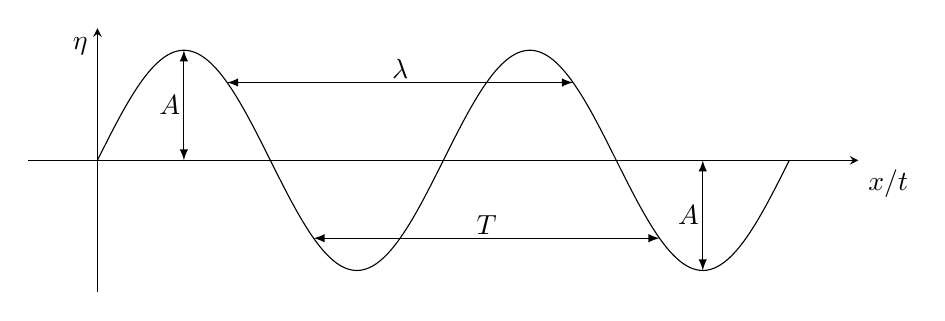
\begin{tikzpicture}
\begin{axis}[
	axis lines=middle,
	enlargelimits=true,
	width=\textwidth,
	axis equal image,
	xmin = 0,
	xmax = 4*pi,
	ymin = -2,
	ymax = 2,
	ylabel = $\eta$,
	xlabel = $x$/$t$,
% 	xtick = {1.57079632679, 3.14159265359, ..., 12.5663706144},
	xtick=\empty,
%  	xticklabels=\empty,
% 	yticklabels={$-\frac{K}{2}$,0,$\frac{K}{2}$},
	%xtick=\empty,
	ytick=\empty,
	every axis x label/.style={at={(current axis.right of origin)},anchor=north west},
	every axis y label/.style={at={(current axis.above origin)},anchor=north east}
	]
\addplot[samples=300,domain=0:4*pi] {2*sin(deg(x))};
\draw[<->,>=latex] (axis cs:pi/2,0) -- (axis cs:pi/2,2) node [midway,label={[xshift=2mm]left:{$A$}}] {};
\draw[<->,>=latex] (axis cs:7*pi/2,0) -- (axis cs:7*pi/2,-2) node [midway,label={[xshift=2mm]left:{$A$}}] {};
\draw[<->,>=latex] (axis cs:3*pi/4,2*0.707106781186548) -- (axis cs:11*pi/4,2*0.707106781186548) node [midway,label={[yshift=-2mm]above:{$\lambda$}}] {};
\draw[<->,>=latex] (axis cs:5*pi/4,-2*0.707106781186548) -- (axis cs:13*pi/4,-2*0.707106781186548) node [midway,label={[yshift=-2mm]above:{$T$}}] {};
\end{axis}
\end{tikzpicture}
\caption{A sinusoidal wave with amplitude $A$, \wavelength $\lambda$, and wave period $T$.}
\label{fig:sinusoid}
\end{figure}
%

We may picture the wave form as defined by Equation~\ref{eq:sinusoid} in an easy
way if we either focus on a fixed position $x$ or a fixed point in time $t$,
see Figure~\ref{fig:sinusoid}.
If we assume a fixed position, we can see the surface elevation evolve through
time at that position. On the other hand, if we assume a fixed point in time, we
can observe surface elevation at all positions at that specific time. The wave's
high point is called a~\emph{crest}, its low point a~\emph{trough}. Because
surface elevation is described by a cosinus function, all crests and all troughs
will have the same elevation. Another effect of the cosinus function is that the
surface elevation is limited by the amplitude $A$. We will call the difference
in elevation between crest and trough the~\emph{wave height}. It is easy to see
that wave height $H$ is defined as $H=2A$.
%Before we move on to waves in three dimensions, we may elaborate on the
%functional relationship between \wavenumber $k$ and angular wave frequency
%$\omega$ as defined by linear wave theory.
% Next, we will look at the
% interdependency between \wavenumber $k$, wave frequency $\omega$, and the
% propagation speed of the wave.
%
\subsection{Phase Velocity}
\label{sec:phase_velocity}
In linear wave theory, the rate at which a particular phase of a wave propagates in space is called
the~\emph{phase velocity}. The phase velocity is a vector and has an associated direction,
the \emph{phase speed} on the other hand refers only to the magnitude of the phase velocity.
The most comprehensible example of phase speed is the rate of propagation of the wave crest.
During one wave period $T$ the wave crest travels a distance equal to the \wavelength $\lambda$.
We may generalize this to other phases than the wave crest. Given a constant phase
\begin{equation*}
  const = kx - \omega t
\end{equation*}
the surface elevation $\eta$ will always be the same. We rewrite the term to
\begin{equation*}
  x = \frac{\omega}{k}t + \frac{const}{k}
\end{equation*}
which gives us all positions $x$ where the wave has the same elevation. These
positions are time-dependent, differentiation gives us phase speed $c$:
\begin{equation*}
  c = \frac{\mathrm dx}{\mathrm dt} = \frac{\omega}{k} = \frac{\lambda}{T}
\end{equation*}

\subsection{The Dispersion Relation}
\label{sec:dispersion_relation}

In the context of water surface waves,~\emph{dispersion} refers to~\emph{frequency dispersion}, which describes
the effect of waves at different wavelengths travelling at different phase speeds. We have seen that
phase speed $c = \lambda/T$ involves \wavelength and frequency, and alternatively $c = \omega/k$
which includes angular frequency and \wavenumber. We focus on the latter formulation for phase speed, because
linear wave theory defines a functional relationship between the two factors involved:
%therefore we will start with the functional relationship
%between angular frequency~$\omega$ and wave number~$k$ as defined by linear wave theory:
\begin{equation}
\label{eq:dispersion_relation}
 \omega^2 = gk\tanh(kd)
\end{equation}
%
where $g$ is the acceleration of earth's gravity and $d$ is the water depth. Equation~\ref{eq:dispersion_relation}
is called the~\emph{dispersion relation}.
There exist two useful approximations of the equation which do not involve the $\tanh$ term:
\begin{itemize}
 \item \emph{Shallow water approximation} - the water depth $d$ is much smaller than the wave length $\lambda$.
 Assume $d \ll \lambda$, then $0 \leq kd \ll 1$ and $\tanh(kd) \approx kd$.
 \item \emph{Deep water approximation} - the water depth $d$ is much larger than the wave length $\lambda$.
 Assume $d \gg \lambda$, then $kd \gg 1$ and $\tanh(kd) \approx 1$.
\end{itemize}
%
The reduced dispersion relations are as follows:
\begin{align*}
%\label{eq:disp_rel_shallow_water}
\omega^2 & = gk^2d && \text{with} & d &< \frac{\lambda}{20}  && \text{Shallow 
water dispersion relation}\\
%\label{eq:disp_rel_deep_water}
\omega^2 & = gk    && \text{with} & d &> \frac{\lambda}{2} && \text{Deep water 
dispersion relation}
\end{align*}
%
Given the dispersion relation approximations for shallow and deep water, the corresponding
phase speeds are:
\begin{align}
 \label{eq:phase_speed_shallow_water} c &= \sqrt{gd} && \text{Shallow water phase speed}\\
  \label{eq:phase_speed_deep_water}   c &= \sqrt{\frac{g}{k}} = \frac{g}{\omega} && \text{Deep water phase speed}
\end{align}
%
According to Equation~\ref{eq:phase_speed_shallow_water}, the phase speed in shallow water depends exclusively
on water depth and gravitational acceleration, there is no connection to \wavelength or frequency.
We may conclude that waves with different \wavelengths travel with the same phase speed, it follows that
shallow water is not dispersive. Phase speed in deep water, on the other hand,
does not relate to water depth, but to \wavelength and frequency, which makes deep water dispersive.
We can expand Equation~\ref{eq:phase_speed_deep_water} to:
%
\begin{equation}
\label{eq:phase_speed_deep_water_l}
 c = \sqrt{\frac{g\lambda}{2\pi}} = \frac{gT}{2\pi}
\end{equation}
%
Looking at Equation~\ref{eq:phase_speed_deep_water_l} we can conclude that phase speed in deep water increases
with \wavelength $\lambda$ ~\emph{and} with wave period $T$. Waves in deep water with large \wavelengths/periods
travel faster than those with smaller ones.

\emph{Note}: In the context of this work we concern ourselves only with the
open ocean, where the water is assumed to be deep. Should occasions arise where
we are required to derive terms and formulas based on phase speed or the
dispersion relation, then we will rely exclusively on the deep water phase speed
and the deep water dispersion relation.
%
\subsection{Three Dimensional Wave}
Until now we were discussing a two-dimensional ocean defined by exactly one sinus wave. As a first
step to get to a more realistic ocean surface representation we will extend Equation~\ref{eq:sinusoid}
to form a wave in three dimensional space. In contrast to Equation~\ref{eq:sinusoid}, where the wave's
travelling direction is fixed, the wave has to be able to travel in an arbitrary direction on a plane.
Moreover, we need to handle two-dimensional input positions. The sinusoid describing surface elevation
in three dimensional space is defined as follows:
\begin{equation}
\label{eq:sinusoid_3d}
 \eta(\mvec{x}, t) = A\cos(\transpose{\mvec{k}}\mvec{x} - \omega t)
\end{equation}
where $\mvec{x} = (x, z)$ denotes the observed point on a plane and $\mvec{k} = (k_x, k_z)$ represents
the travelling direction of the wave. The \wavenumber $k$ of~\emph{\wavevector} $\mvec{k}$ is determined by
the \wavevector's magnitude:
\begin{equation*}
 k = \norm{\mvec{k}}
\end{equation*}
Because of the dispersion relation, all waves of same magnitude $k$ share the
same angular frequency $\omega$.

\subsection{Complex Exponential Wave Form}
%
Before we start handling a large number of sinusoids, we will improve our
notation to make it more compact. In order to do that we employ~\emph{Euler's
formula}~\citep{Euler:1748}:
\begin{align}
\label{eq:euler_positive} e^{ix} &= \cos{x} + i\sin{x} && x \in \mathbb{R} \\
\label{eq:euler_negative} e^{-ix} &= \cos{x} - i\sin{x} && x \in \mathbb{R}
\end{align}
%
We may extract both the real and the imaginary part separately:
\begin{align*}
 \cos{x} &= \Re\{e^{ix}\} \\
 \sin{x} &= \Im\{e^{ix}\}
\end{align*}
where $\Re$ denotes the real part of the exponential and $\Im$ the
complex one. Alternatively we may solve Equations~\ref{eq:euler_positive}
and~\ref{eq:euler_negative} as a pair in the variables $\cos{x}$ and $\sin{x}$:
\begin{align*}
 \cos{x} &= \frac{e^{ix}+e^{-ix}}{2}\\
 \sin{x} &= \frac{e^{ix}-e^{-ix}}{2i}\\
\end{align*}
Now we are able to rewrite our current formulation of a sinusoid in three
dimensional space from Equation~\ref{eq:sinusoid_3d} as an exponential:
%
\begin{align}
\label{eq:sinusoid_exponential_sa} \eta(\mvec{x}, t) &=
\Re\{A\mathrm{e}^{\mathrm{i}[\transpose{\mvec{k}}\mvec{x} -{\omega}t]}\} \\
\intertext{or equivalent}
 p &= A\mathrm{e}^{\mathrm{i}[\transpose{\mvec{k}}\mvec{x} -
{\omega}t]} \nonumber \\
 \eta(\mvec{x}, t) &= \frac{p+p^*}{2} \nonumber
\end{align}
%
where $p^*$ denotes the~\emph{complex conjugate} of $p$. From now on we will
omit the explicit $\Re$ in equations expressing $\eta$, because surface
elevation is a real number.
%
\subsection{Sum of Waves}
Now that we have a description of waves in three-dimensional space, we need to
enhance the description of the ocean surface. It is obvious that the ocean does
not consist of only one wave travelling, but of an infinite number of waves with
different lengths and directions. Because we still find ourselves in the realm
of~\emph{linear} wave theory, we may reach an adequate solution
by~\emph{combination}. A linear combination of solutions constitutes a valid
solution as well.

Each combination of amplitude $A$, \wavevector $\mvec{k}$ and wave frequency
$\omega$ identifies one particular wave. As a next step we get rid of the
restriction of one single amplitude $A$ for all wave components. We replace the
constant amplitude $A$ with $a(\mvec{k})$ in order to create a dependency
between \wavevector and wave amplitude. Furthermore, because of the dispersion
relation, we can express frequency as a function of the \wavevector, $\omega =
\omega(\mvec{k})$. Now we are able to rewrite
Equation~\ref{eq:sinusoid_exponential_sa} as follows:
\begin{equation}
\label{eq:sinusoid_exponential_ak_wk}
\eta(\mvec{x}, t) =
a(\mvec{k})\mathrm{e}^{\mathrm{i}(\transpose{\mvec{k}}\mvec{x}-
\omega(\mvec{k})t)}
\end{equation}
%
We already mentioned that we seek a solution by linear combination. Based on
Equation~\ref{eq:sinusoid_exponential_ak_wk} we may express surface
elevation as an infinite sum of sinusoids:
\begin{equation}
\label{eq:surface_elevation_akwt}
 \eta(\mvec{x}, t) = \iint_{\mvec{k}}
a(\mvec{k})~\mathrm{e}^{\mathrm{i}(\transpose{\mvec{k}}\mvec{x}-
\omega(\mvec{k})t)}~\mathrm{d}\mvec{k}
\end{equation}
where $a(\mvec{k})$ is called the~\emph{amplitude spectrum} of
$\eta(\mvec{x}, t)$.
According to \citet{book:kinsman2002wind} it is more expedient to
represent the vertical displacement of the water surface by~\emph{Generalized
Fourier Transforms} \citep{book:lighthill1958}.
%We may rewrite the sea surface in two spatial dimensions and one time dimension as follows:
Thus, \citeauthor{book:kinsman2002wind} transforms Equation~\ref{eq:surface_elevation_akwt}
into a sea surface representation with two spatial dimensions and one time dimension:
%
\begin{equation}
\label{eq:surface_elevation_bkwt}
 \eta(\mvec{x}, t) = \iint_{\mvec{k}}\int_{\omega} B(\mvec{k},
\omega)~\mathrm{e}^{\mathrm{i}(\transpose{\mvec{k}}\mvec{x}-
\omega t)}~
\mathrm{d}\mvec{k}~\mathrm{d}\omega
\end{equation}
where the $\mvec{k}$ integration is over all \wavenumber space and the $\omega$
integration is over all frequencies. $B(\mvec{k},\omega)$ is called the
three dimensional amplitude spectrum of $\eta(\mvec{x}, t)$. Notice the missing
dependency of $\omega$ on $\mvec{k}$ in the exponent, it is the responsibility
of $B(\mvec{k},\omega)$ to model that relationship.
We may integrate separately over all frequencies to obtain the two-dimensional
amplitude spectrum $B(\mvec{k}, t)$:
%
\begin{equation}
\label{eq:surface_elevation_bkt}
 B(\mvec{k}, t) = \int_{\omega} B(\mvec{k},
\omega)~\mathrm{e}^{-\mathrm{i}\omega t}~\mathrm{d}\omega
\end{equation}
%
Alternatively, we may integrate over all \wavenumbers to obtain the one dimensional
amplitude spectrum $B(\mvec{x}, \omega)$:
%
\begin{equation}
\label{eq:surface_elevation_bwt}
 B(\mvec{x}, \omega) = \iint_{\mvec{k}} B(\mvec{k},
\omega)~\mathrm{e}^{\mathrm{i}\transpose{\mvec{k}}\mvec{x}}~\mathrm{d}\mvec{k}
\end{equation}
%
Thus, we may rewrite Equation~\ref{eq:surface_elevation_bkwt} in terms of
Equation~\ref{eq:surface_elevation_bkt} and Equation~\ref{eq:surface_elevation_bwt}:
%
\begin{equation}
\label{eq:surface_elevation_bk}
  \eta(\mvec{x}, t) = \iint_{\mvec{k}} B(\mvec{k},t)~\mathrm{e}^{\mathrm{i}\transpose{\mvec{k}}\mvec{x}}~\mathrm{d}\mvec{k}
  = \int_{\omega} B(\mvec{x},\omega)~\mathrm{e}^{-\mathrm{i}\omega t}~\mathrm{d}\omega
\end{equation}
%
% We rewrite Equation~\ref{eq:surface_elevation_bkwt} as
% %
% \begin{equation}
% \label{eq:surface_elevation_bw}
% \eta(\mvec{x}, t) = \int_{\omega} B(\mvec{x},\omega)
% ~\mathrm{e}^{-\mathrm{i}\omega t}~\mathrm{d}\omega
% \end{equation}
%
\section{The Specification of a Random Sea}
\label{sec:random_sea}
%
Equation~\ref{eq:surface_elevation_bk} may be able to describe the ocean
surface, but at the cost of deducing an amplitude spectrum for each observed
point on the sea surface, a both tedious and unfeasible task. At
this point we are in need of a general description of the amplitude spectrum
which is valid at all points $\mvec{x}$ and times $t$.
Fortunately, modern physical oceanography is
based on exactly such a formulation, which has been developed by \citet{Neumann:1966}.
% We will refer to said formulation as \emph{Pierson-Neumann theory} throughout
% the remainder of this document.

\citeauthor{Neumann:1966} combine oceanography, physics and stochastics in order
to describe the ocean surface. A fundamental assumption of their theory is that
surface disturbance is formed from many contributions caused by relatively
unrelated forces at different times. Therefore it is reasonable to presume that
the elements in the summation of Equation~\ref{eq:surface_elevation_bk} are
statistically independent.
% As a consequence the central limit theorem \cite{book:ctm:fischer} with the
% resulting distribution being a Gaussian is applied. The result is
% a \emph{spatially homogeneous} and \emph{temporally stationary} Gaussian random
% process which models a wind driven ocean surface.
\citeauthor{Neumann:1966} model the wind driven ocean surface as a
\emph{spatially homogeneous} and \emph{temporally stationary} Gaussian random
process~\citep{book:grimmett2001}. The random process is said to be
\emph{homogeneous}, because it is independent of the origin selected for
positions $\mvec{x}$, furthermore it is \emph{stationary} since absolute time is
irrelevant, only time difference matters.
%
\subsection{The Energy Spectrum}
\label{sec:energy_spectrum}
Given a spatially homogeneous and temporally stationary wave field, and a
respective three dimensional amplitude spectrum $B(\mvec{k},\omega)$, then we
may write:
\begin{equation}
\label{eq:energy_spectrum_3d}
 \Theta(\mvec{k}, \omega) = \frac{B(\mvec{k}, \omega)^2}{2} = 
\overline{B(\mvec{k}, \omega)B^{*}(\mvec{k}, \omega)}
\end{equation}
where the $\overline{B}$ operator denotes the mean and
$\Theta(\mvec{k},\omega)$ represents the~\emph{mean square displacement} of
wave amplitude $B(\mvec{k},\omega)$. The mean square displacement of a wave
is connected to wave energy $E_w$ as follows:
%
\begin{equation}
\label{eq:wave_energy_single}
 E_w = \rho g~\Theta(\mvec{k},\omega)
\end{equation}
%
where $\rho$ is the water density and $g$ the accleration of earth's gravity.
Equation~\ref{eq:wave_energy_single} is the reason $\Theta(\mvec{k},\omega)$
in literature is referred to as the three dimensional~\emph{energy spectrum}
associated with $B(\mvec{k},\omega)$. Now we are able to define mean surface
energy $E_s$ based on combined wave energy:
%
\begin{equation}
\label{eq:wave_energy_3d}
 E_s = \rho g~\iint_{\mvec{k}}\int_{\omega}\Theta(\mvec{k},\omega)
~\mathrm{d}\mvec{k}~\mathrm{ d}\omega
\end{equation}
%
Looking back at Equation~\ref{eq:wave_energy_single}, which makes wave energy
dependent on the mean square displacement of wave amplitudes, we may deduce that
mean surface energy is dependent on the~\emph{mean square surface displacement},
denoted as $\overline{\eta^2}$. Therefore, we may write:
%
\begin{equation}
\label{eq:mean_square_eta}
\overline{\eta^2} = \iint_{\mvec{k}}\int_{\omega}\Theta(\mvec{k},\omega)
~\mathrm{d}\mvec{k}~\mathrm{d}\omega
\end{equation}
%
\\
Later on we will be in need of energy spectrum formulations which have a lower
dimensionality than the three dimensional $\Theta(\mvec{k},\omega)$. As such,
we introduce the two-dimensional energy spectrum, in literature known
as~\emph{\wavenumber spectrum}, which is defined as follows:
\begin{equation}
\label{eq:energy_spectrum_2d}
 \Theta(\mvec{k}) = \int_{\omega} \Theta(\mvec{k}, \omega)~\mathrm{d}\omega
\end{equation}
The \wavenumber spectrum gives the contribution to the wave energy arising from
wave components with \wavenumber $k$ dependent on \wavevector $\mvec{k}$,
irrespective of the frequencies $\omega$ associated with that \wavenumber. In
contrast, the one dimensional energy spectrum, in literature known
as~\emph{frequency spectrum}, is defined as follows:
\begin{equation}
\label{eq:energy_spectrum_1d}
 \Theta(\omega) = \int_{\mvec{k}} \Theta(\mvec{k}, \omega)~\mathrm{d}\mvec{k}
\end{equation}
The frequency spectrum gives the contributions to the energy coming from each
frequency $\omega$, irrespective of the \wavenumbers associated with that
frequency.

\emph{Note}:
The energy spectrum as presented is severely restricted in its
capabilities to model a~\emph{dynamic} ocean. Dynamic, in this context, means an
ocean which may start as a perfectly flat surface, is actuated to a fully
developed sea by wind, decays back into a near motionless state, and so on and
so forth. The energy spectrum as discussed only models waves on an ocean with
infinite extend over which a uniform wind has been blowing forever. In context
of this document such a model of the ocean is sufficient, there is no need to
simulate the actual generation and decay of waves over time.

\subsection{The Random Process}
\label{sec:random_process}
Based on the wave energy spectrum, \citet{Neumann:1966} describe the sea surface
as a Gaussian random process.
As such, we are not dealing with one concrete ocean surface $\eta$, but with an
\emph{ensemble} of different sea surfaces $\{\eta\}$, each associated with its
own probability to be actually realised. Because the random process is a
Gaussian one, it has an associated Gaussian Distribution with mean
$\mathrm{E}[\eta]$ and variance $\mathrm{Var}[\eta] = \sigma^2$. Considering a
sea surface in combination with linear wave theory, where a symmetry between
troughs and crests is a given, the mean is easily found:
\begin{equation*}
 \mathrm{E}[\eta] = 0
\end{equation*}
%
Moreover, all spectral components $B(\mvec{k},\omega)$ are assumed to be
\emph{statistically independent}, each with mean zero and variance $\Theta(\mvec{k},\omega)$,
therefore the variance of all components combined is:
\begin{equation*}
\label{eq:random_process_variance}
\mathrm{Var}[\eta] = \sigma^2 = \iint_{\mvec{k}}
\int_{\omega}\Theta(\mvec{k},\omega)~\mathrm{d}\mvec{k}~\mathrm{ d}\omega
\end{equation*}
which is the same as Equation~\ref{eq:mean_square_eta}. The variance
$\sigma^2$ is equal the mean square surface elevation $\overline{\eta^2}$. With
mean and variance at hand we may write the Gaussian Distribution that the
values of sea surface elevation are drawn from:
\begin{equation}
\label{eq:gaussian_dist}
 pr[\eta] = \frac{1}{\sqrt{2\pi\sigma^2}}~\mathrm{e}^{-\frac{\eta^2}{2\sigma^2}}
\end{equation}
Note that neither position nor time appear in the distribution, because the
process is modeled as spatially and temporally invariant.
% We already mentioned that Pierson-Neumann theory does not represent surface
% elevation $\eta$ as one single function, but as an ensemble of functions
% $\{\eta\}$. The ensemble contains an infinite number of different sea surfaces,
% each with its own probability of actually being realised.
As of now, we may formulate surface elevation as a realisation of a stochastic process:
\begin{equation}
\label{eq:surface_elevation_gauss}
 \eta(\mvec{x}, t) = \iint_{\mvec{k}}\int_{\omega} \xi
~\mathrm{e}^{\mathrm{i}(\transpose{\mvec{k}}\mvec{x}-
\omega t)}~
\mathrm{d}\mvec{k}~\mathrm{d}\omega
\end{equation}
where $\xi$ is a Gauss distributed variable with mean $\mathrm{E}[\eta] = 0$,
and variance $\mathrm{Var}[\eta] = \sigma^2$ as defined by the energy spectrum
$\Theta(\mvec{k}, \omega)$. One may realize that in context of this formulation
of sea surface elevation, the energy spectrum is the key to believable
ocean surfaces, as it needs to be able to model the underlying physical
processes to give realistic results.\\

% At this point we have to face the reality of oceanographic research, which does 
% not provide us with any three dimensional energy spectra 
% $\Theta(\mvec{k},\omega)$. On the other hand, we are given a set of 
% parametric one dimensional frequency spectra $\Theta(\omega)$ which we are not 
% able to use as-is, because they do not contain any information about the 
% travelling direction of waves, and therefore are not able to simulate 
% surface elevation with two-dimensional positions $\mvec{x}$ as input.
From an algorithmic point of view we should not use three dimensional
energy spectra $\Theta(\mvec{k},\omega)$ to synthesize the ocean surface, as
the computational cost of \FourierTransforms in three dimensions would simply
be too high.
On the other hand, we are unable to employ one dimensional frequency spectra
$\Theta(\omega)$ as-is, because they do not contain any information about
the  travelling direction of waves, and therefore are not able to compute 
surface elevation with two-dimensional positions $\mvec{x}$ as input.
Hence, we have to settle for the two-dimensional \wavenumber spectrum
$\Theta(\mvec{k})$ as basis. We may write surface elevation as follows:
\begin{equation}
\label{eq:surface_elevation_gauss_2d}
 \eta(\mvec{x}, t) = \iint_{\mvec{k}} 
\xi~\mathrm{e}^{-\mathrm{i}\omega(\mvec{k}) t}
~\mathrm{e}^{\mathrm{i}\transpose{\mvec{k}}\mvec{x}}~\mathrm{d}\mvec{k}
\end{equation}
where, in line with Equation~\ref{eq:surface_elevation_gauss}, $\xi$ is 
a Gauss distributed variable with mean $\mathrm{E}[\eta] = 0$ and
variance $\mathrm{Var}[\eta] = \sigma^2$ defined by the energy spectrum
$\Theta(\mvec{k})$. Moreover, for animation purposes, we add the term 
$\mathrm{e}^{-\mathrm{i}\omega(\mvec{k}) t}$ to explicitely handle 
time $t$, because the two-dimensional \wavenumber spectrum has no notion of 
it. Equation~\ref{eq:surface_elevation_gauss_2d} represents a two-dimensional 
\InvFourierTransform of Fourier components 
$\xi\mathrm{e}^{-\mathrm{i}\omega(\mvec{k}) t}$. For the remainder of the 
document, Equation~\ref{eq:surface_elevation_gauss_2d} will be the basis for all 
further discussions of specific wave spectrum models. Moreover, in 
Section~\ref{sec:wave_spectra} we will discuss the conversion of the 
more common one dimensional frequency spectra $\Theta(\omega)$ into two 
dimensional \wavenumber spectra $\Theta(\mvec{k})$ for our practical usage.
%
\section{Discretisation}
\label{sec:random_sea_discretisation}
For computer graphics applications we are in need of a discrete approximation 
of surface elevation as defined by 
Equation~\ref{eq:surface_elevation_gauss_2d}, 
which gives acceptable results as well as computes said results in a reasonable 
amount of time. We may write a rough sketch of such a discrete formulation like 
the following:
\begin{equation}
\label{eq:surface_elevation_sketch}
 \eta(\mvec{x}, t) = \sum_{\mvec{k}} 
\xi~\mathrm{e}^{-\mathrm{i}\omega(\mvec{k}) t}
~\mathrm{e}^{\mathrm{i}\transpose{\mvec{k}}\mvec{x}}
\end{equation}
Equation~\ref{eq:surface_elevation_sketch} represents a \InvDiscreteFourierTransform of Fourier components 
$\xi\mathrm{e}^{-\mathrm{i}\omega(\mvec{k}) t}$, which we are able to compute in 
a very efficient manner by means of the \FastFourierTransform, 
~\emph{\FFT} in short. The interested reader may find extensive discussions of 
the \DiscreteFourierTransform and the Fast Fourier algorithm
in \cite{book:bracewell2000fourier} and \cite{book:numericalrecipes}.

Employing the FFT algorithm may ease our concerns with regard to performance, but 
we still have to make sure we compute an as good as possible approximation of 
Equation~\ref{eq:surface_elevation_gauss_2d}. Since our model for surface 
elevation is based on wave energy, the best way forward seems to be that we 
choose a finite range of \wavevectors $\mvec{k}$ such that they are 
representative of the whole energy $\mathrm{Var}[\eta]$ as defined by $\Theta(\mvec{k})$. 
Because \wavevectors $\mvec{k}$ are related to \wavelength, they are also 
related to the spatial domain, and as such to positions $\mvec{x}$. Hence, the 
quality of our approximation depends on how we discretise both the spatial 
domain into a finite set of positions $\mvec{x}$ and the \wavevector domain 
into a finite set of \wavevectors $\mvec{k}$.
%
\subsection{Domain Discretisation}
\label{sec:domain_discretisation}
%
We define the sea surface we want to synthesize as a rectangular area, with $L$
and $K$ denoting width and height in meters respectively. Moreover, we
discretise said rectangle into a grid with horizontal resolution $N$ and
vertical resolution $M$, where both $N$ and $M$ shall be an integer which can
be represented as a power of two. Therefore we will define sea surface elevation 
at $N\times M$ discrete points. We will denote the horizontal and vertical
distance between consecutive grid points as follows:
\begin{align*}
 \Delta x = \frac{L}{N} && \Delta z = \frac{K}{M}
\end{align*}
We compute surface elevation at the following points:
\begin{equation}
\label{eq:spatial_domain}
 \mvec{x} = (x,z)~\in~\{(\alpha\Delta x,\beta\Delta y)|
-\frac{N}{2}\leq\alpha<\frac{N}{2},-\frac{M}{2}<\beta\leq\frac{M}{2}\}
\end{equation}
where $\alpha$ and $\beta$ are integers. At first glance the choice of interval
for positions~$\mvec{x}$ may seem arbitrary, but it will allow us to make a
direct connection to the \wavevector domain later on.
To simplify matters we will handle a square area instead of a rectangular one,
thus:
\begin{align*}
%\label{eq:square_area}
 N = M && L = K &&\Rightarrow \Delta x = \Delta z
\end{align*}
%
Based on the~\emph{Nyquist-Shannon sampling
theorem} \citep{book:bracewell2000fourier} we are able to compute the minimum and
maximum \wavelengths which are reconstructible without loss of information.
We may write said minimum and maximum \wavelengths as follows:
\begin{align*}
 \lambda_{min} = 2\Delta x && \lambda_{max} = \sqrt{2}~\Delta x~\frac{N}{2}
\end{align*}
%
%
\begin{figure}
\centering
%\tikzset{external/force remake}
\begin{tikzpicture}
% let both axes use the same layers
\pgfplotsset{set layers}
\begin{axis}[
    grid=major,
    enlargelimits=false,
    scale only axis,
    axis equal=true,
%    width = \textwidth,
    xmin=-5,
    xmax=5,
    ymin=-5,
    ymax=5,
    xtick = {-4,0, 4},
    ytick = {-4,0, 4},
    xticklabels={$-\frac{N}{2}$,0,$\frac{N}{2}$},
    yticklabels={$-\frac{M}{2}$,0,$\frac{M}{2}$},
    xlabel={$\alpha$},
    ylabel={$\beta$},
    ]
\addplot graphics[
    xmin=-5,
    xmax=5,
    ymin=-5,
    ymax=5,
]
{figures/ifft_spatial_domain_odd};
\end{axis}
%
\begin{axis}[
    enlargelimits=false,
    scale only axis,
    axis equal=true,
%    width = \textwidth,
    xmin=-5,
    xmax=5,
    axis x line* = top,
    ymin=-5,
    ymax=5,
    axis y line* = right,
    xtick = {-4,0, 4},
    ytick = {-4,0, 4},
    xticklabels={$-\frac{L}{2}$,0,$\frac{L}{2}$},
    yticklabels={$-\frac{K}{2}$,0,$\frac{K}{2}$},
    xlabel = {$\alpha\cdot\Delta x$},
    ylabel={$\beta\cdot\Delta z$},
    ]
\end{axis}
\end{tikzpicture}
\caption{The spatial domain in terms of index pairs
$(\alpha,\beta)$ and associated coordinate pairs $(\alpha\Delta x,\beta\Delta z)$.}
\label{fig:spatial_domain}
\end{figure}
%
%
Figure~\ref{fig:spatial_domain} depicts the spatial domain as defined
by resolution and size, including horizontal and vertical grid point distances,
as well as minimum and maximum \wavelengths.

\begin{figure}
\centering
%\tikzset{external/force remake}
\begin{tikzpicture}
% let both axes use the same layers
\pgfplotsset{set layers}
\begin{axis}[
    grid=major,
    enlargelimits=false,
    scale only axis,
    axis equal=true,
%    width = \textwidth,
    xmin=-5,
    xmax=5,
    ymin=-5,
    ymax=5,
    xtick = {-4,0, 4},
    ytick = {-4,0, 4},
    xticklabels={$-\frac{N}{2}$,0,$\frac{N}{2}$},
    yticklabels={$-\frac{M}{2}$,0,$\frac{M}{2}$},
    xlabel={$\alpha$},
    ylabel={$\beta$},
    ]
\addplot graphics[
    xmin=-5,
    xmax=5,
    ymin=-5,
    ymax=5,
]
{figures/ifft_wave_vector_domain_odd};
\end{axis}
%
\begin{axis}[
    enlargelimits=false,
    scale only axis,
    axis equal=true,
%    width = \textwidth,
    xmin=-5,
    xmax=5,
    axis x line* = top,
    ymin=-5,
    ymax=5,
    axis y line* = right,
    xtick = {-4,0, 4},
    ytick = {-4,0, 4},
    xticklabels={$-\frac{\pi N}{L}$,0,$\frac{\pi N}{L}$},
    yticklabels={$-\frac{\pi M}{K}$,0,$\frac{\pi M}{K}$},
    xlabel = {$\alpha\cdot\Delta k_x$},
    ylabel={$\beta\cdot\Delta k_z$},
    ]
 %
\end{axis}
\end{tikzpicture}
\caption{The \wavevector domain in terms of index pairs $(\alpha,\beta)$ and
associated coordinate pairs $(\alpha\Delta k_x,\beta\Delta k_z)$.}
\label{fig:wave_vector_domain}
\end{figure}
%
With $\lambda_{min}$ and $\lambda_{max}$ at hand we may compute the
corresponding \wavenumbers:
\begin{align}
\label{eq:kmin_kmax}
 k_{min} = \frac{2\pi}{\lambda_{min}} && k_{max} = \frac{2\pi}{\lambda_{max}}
\end{align}
%
Analogous to the spatial domain, we have to define the horizontal and vertical 
distance between consecutive grid points for the \wavevector domain. We denote 
said distances as follows:
\begin{align}
\label{eq:delta_kx_delta_ky}
 \Delta k_x = \Delta k_z = \frac{2\pi}{L} = \frac{2\pi}{K}
\end{align}
%
Given $\Delta k_x$ and $\Delta k_z$, we will define \wavevectors $\mvec{k}$ in 
the same fashion as Equation~\ref{eq:spatial_domain} defines spatial positions 
$\mvec{x}$:
\begin{equation}
\label{eq:wave_vector_domain}
 \mvec{k} = (k_x,k_z)~\in~\{(\alpha\Delta k_x,\beta\Delta k_z)|
-\frac{N}{2}\leq\alpha<\frac{N}{2},-\frac{M}{2}<\beta\leq\frac{M}{2}\}
\end{equation}
where $\alpha$ and $\beta$ are integers.
%
%As one may see in Figure~\ref{fig:wave_vector_domain}, the \wavevector domain 
%is centered. \Wavenumber $k = 0$ is at the center, and $|k|$ grows while we 
%move outwards, towards the domain border.
We know that the relation between \wavelength and \wavenumber is an inverse one,
while $\norm{\mvec{k}}$ increases, \wavelength $\lambda$ decreases. Therefore we find the larger
\wavelengths near the domain center, and the smaller ones near the domain border.
%We may ignore the center element 
%with \wavenumber $k = 0$, which maps to wave length $\lambda = \infty$, because 
%$\Theta(\mvec{k})$ is always equal zero for \wavevector $\mvec{k} = (0, 0)$.
Figure~\ref{fig:wave_vector_domain} shows the \wavevector domain as defined
by Equation~\ref{eq:wave_vector_domain}, including \wavevectors which are exact
representatives for \wavenumbers $k_{min}$ and $k_{max}$. As expected, $k_{min}$
is found at the domain border, and $k_{max}$ near the domain center.
We may rewrite \wavenumbers $k_{min}$ and $k_{max}$ from
Equation~\ref{eq:kmin_kmax} to the following:
\begin{align*}
 k_{max} &= \sqrt{2}\Delta k_x = \sqrt{2}\Delta k_z = \sqrt{2}\frac{2\pi}{L} = \sqrt{2}\frac{2\pi}{K} \\
 k_{min} &= \frac{\pi N}{L} = \frac{\pi M}{K}
\end{align*}
Hence, by choosing surface dimensions $L$ and $K$ we implicitely determine the 
maximum \wavelength we are able to include in our computation.
With surface dimensions $L$ and $K$ fixed, we choose the number of 
samples $N$ and $M$, knowing that they will define the smallest \wavelength 
representable by \wavevectors $\mvec{k}$.

Later on we will see that the 
distribution of wave energy among \wavevectors is highly dependent on the 
actual wave spectrum, as well as on the input parameters to the wave spectrum.
Wave energy may be focused in a very narrow range of \wavevectors, or be wide spread 
among a large portion of the entire \wavevector spectrum. As a consequence, 
sometimes it is necessary to choose multiple sets of \wavevectors 
$\mvec{k}$ which complement one another, and to combine the results in order 
to get satisfactory results.
%
\subsection{Energy Discretisation}
%
We have discretised the \wavevector domain into a finite set of \wavevectors, 
where $\pm k_{min}$ represent the largest positive and negative \wavenumbers on 
the horizontal and vertical axes. Since we seek a representative approximation 
of whole wave energy $\mathrm{Var}[\eta]$ based on our finite set of \wavevectors, we may 
start by limiting the respective integral with $\pm k_{min}$:
\begin{equation}
\label{eq:variance_int_approx_limited}
\mathrm{Var}[\eta] = \iint_{\mvec{k}}\Theta(\mvec{k})~\mathrm{d}\mvec{k}
\approx\int_{-k_{min}}^{k_{min}}\int_{-k_{min}}^{k_{min}}\Theta(\mvec{k}
)~\mathrm{d}\mvec{k}
\end{equation}
We may rewrite the approximation in 
Equation~\ref{eq:variance_int_approx_limited} as a sum of integrals:
%
\begin{equation}
\label{eq:variance_int_approx_sums}
 \mathrm{Var}[\eta] = \int_{-k_{min}}^{k_{min}}\int_{-k_{min}}^{k_{min}}\Theta(\mvec{k}
)~\mathrm{d}\mvec{k} = \sum_{\alpha}\sum_{\beta}\int_{\Delta k_x}\int_{\Delta 
k_z}\Theta(\mvec{k})~\mathrm{d}\mvec{k}
\end{equation}
%
where $\alpha$ and $\beta$ are the indices from 
Equation~\ref{eq:wave_vector_domain}, and $\Delta k_x$ and $\Delta k_z$ 
represent the distances between grid points as defined by 
Equation~\ref{eq:delta_kx_delta_ky}. Alternatively, we may compute an 
approximation of wave energy in a pure discrete way. Let 
$\mvec{k}_{\alpha,\beta}$ be the \wavevectors defined by 
Equation~\ref{eq:wave_vector_domain}, then:
%
\begin{equation}
\label{eq:variance_naive_sum}
 \mathrm{Var}[\eta] = \sum_{\alpha}\sum_{\beta}\Theta(\mvec{k}_{\alpha,\beta})
\end{equation}
%
By combining Equation~\ref{eq:variance_int_approx_sums} 
and~\ref{eq:variance_naive_sum} we get:
%
\begin{equation}
 \Theta(\mvec{k}_{\alpha,\beta}) = \int_{\Delta k_x}\int_{\Delta 
k_z}\Theta(\mvec{k})~\mathrm{d}\mvec{k} \approx 
\Theta(\mvec{k}_{\alpha,\beta})\Delta k_x\Delta k_z
\end{equation}
Now we may write our approximation of the whole wave energy as a simple sum:
\begin{equation}
\label{eq:variance_discrete}
 \mathrm{Var}[\eta] = \sum_{\alpha}\sum_{\beta}\Theta(\mvec{k}_{\alpha,\beta})\Delta k_x 
\Delta k_z
\end{equation}
%
\subsection{Random Amplitudes}
\label{sec:random_amplitudes}
Recall that wave energy is defined as the mean square of the wave amplitude, so,
given wave energy $\Theta(\mvec{k})$, we may compute wave amplitude 
$B(\mvec{k})$ as follows:
\begin{equation*}
 B(\mvec{k})^2 = 2\Theta(\mvec{k})
\end{equation*}
We may convert to a discrete formulation based on 
Equation~\ref{eq:variance_discrete}:
\begin{equation*}
 B(\mvec{k}_{\alpha,\beta})^2 = 2\Theta(\mvec{k}_{\alpha,\beta})\Delta k_x 
\Delta k_z
\end{equation*}
As described in Section~\ref{sec:random_process}, in order to generate random 
wave amplitudes, we employ a Gaussian Distribution with mean $\mathrm{E}[\eta] 
= 0$ and variance $\mathrm{Var}[\eta]$ defined by the energy spectrum
$\Theta(\mvec{k})$. Since all Gaussian Distributions may be written based on 
the Standard Normal Distribution, we are able to write surface elevation as 
follows:
\begin{equation*}
 \eta(\mvec{x}, t) = 
\sum_{\alpha}\sum_{\beta}\frac{1}{\sqrt{2}}(\xi_r+\mathrm{i}\xi_i)\sqrt{B(\mvec{
k}_{\alpha,\beta})^2}~\mathrm{e}^{-\mathrm{i}\omega(\mvec{k}_{\alpha,\beta}) 
t}~\mathrm{e}^{\mathrm{i}\transpose{\mvec{k}_{\alpha,\beta}}\mvec{x}}
\end{equation*}
where $\xi_r$ and $\xi_i$ are random scalars drawn from the Standard Normal Distribution.
We will drop indices $\alpha$ and $\beta$ and give 
a formulation in terms of wave energy $\Theta(\mvec{k})$ and our finite set of 
\wavevectors $\mvec{k}$:
\begin{equation}
\label{eq:surface_elevation_discrete}
 \eta(\mvec{x}, t) = 
\sum_{\mvec{k}}\frac{1}{\sqrt{2}}(\xi_r+\mathrm{i}\xi_i)
\sqrt{2\Theta(\mvec{k})\Delta k_x \Delta k_z} 
~\mathrm{e}^{-\mathrm{i}\omega(\mvec{k})t}
~\mathrm{e}^{\mathrm{i}\transpose{\mvec{k}}\mvec{x}}
\end{equation}
%
We have found a discrete approximation of surface elevation which is fast to 
compute and is able to give satisfactory results as long as we choose one or 
more sets of \wavevectors $\mvec{k}$ wisely. We will now move on and discuss
parametric wave energy models, because those constitute the basis for the
generation of visually pleasing as well as plausible ocean surfaces.
%
\section{Wave Spectra}
\label{sec:wave_spectra}
Oceanographic literature provides us with a large set of different wave spectra
to choose from \citep{Komen:1996}. For our implementation, we decided to pick a
small number of wave spectrum models which, one, are well established in
oceanographic research, and, two, allow us to reproduce a wide variety of ocean
surfaces. We will elaborate on the latter point in Chapter~\ref{ch:summary},
where we discuss the visual results obtained by the different wave spectra.
For now let us focus on the models themselves.
%We will elaborate on the visual results obtained by the different
%wave spectra in Chapter~\ref{ch:summary}. For now let us focus on the models
%themselves.
We will start with a pair of one dimensional frequency spectra most often found
and referenced in oceanographic literature. As said frequency spectra are
one dimensional, we need to convert them into two-dimensional \wavenumber
spectra, as only the latter form allows us to actually synthesize a finite area
of a virtual ocean surface. Thus, first, we follow up with a description of how
to augment one dimensional frequency spectra with directional information, and
second, we show how to make sure to preserve integral equality between
different wave spectrum domains, i.e. how to convert from frequency based wave
energy to \wavenumber based energy with correct scaling.
Last, we discuss three more wave spectra, where each of them already includes a
distinct model for the directional distribution of wave energy.
% 
% we follow up with a description of how to augment them with
% directional information to obtain two-dimensional wavenumber spectra. Only the
% latter form allows us to actually synthesize a finite area of a virtual ocean
% surface. Next, we show how to make sure to preserve integral equality between
% different wave spectrum domains i.e. how to convert from frequency based wave
% energy to wavenumber based energy with correct scaling.
% 
% We will start by discussing two well known one dimensional
% frequency spectra and how to augment them with directional information to obtain
% two-dimensional wavenumber spectra. Only the latter form allows us to actually
% synthesize a finite area of a virtual ocean surface.
% Next, we show how to make sure to preserve integral equality between
% different wave spectrum domains i.e. how to convert from frequency based wave
% energy to wavenumber based energy, with correct scaling.
% Last, we discuss three more wave spectra, two from oceanographic research and
% one from computer graphics, where each already includes a model for the
% directional distribution of wave energy.
%
\subsection{Pierson Moskowitz Spectrum}
\label{sec:pierson_moskowitz}
%
The Pierson Moskowitz spectrum \citep{article:PiersonMoskowitz1964} is a well 
known and widely used one dimensional frequency spectrum based on data aquired 
by weather ships in the North Atlantic Ocean. At the time it was introduced, 
it was expressed in terms of wind speed as follows:

\begin{equation}
%\label{eq:pierson_moskowitz_old}
\label{eq:pierson_moskowitz_theta_old}
 \Theta(\omega) = \frac{\alpha
g^2}{\omega^5}~\exp\left[-\beta\left(\frac{g}{U_{19.5}}\frac{1}{\omega}
\right)^4\right ]
\end{equation}
with
\begin{align*}
\alpha = 8.1 \times 10^{-3} && \beta = 74 \times 10^{-1}
\end{align*}
where $U_{19.5}$ is the wind speed at a height of 19.5 meters above the sea
surface, the height of the anemometers used by Pierson and Moskowitz. Further
analysis of the data \citep{alves:2003} brought to light the subsequent
relationship between wind speed and peak frequency $\omega_p$:
\begin{equation*}
 \beta\left(\frac{g}{U_{19.5}}\right)^4 = \frac{5}{4}~\omega_p^4
\end{equation*}
which lead to a rephrasing of Equation~\ref{eq:pierson_moskowitz_theta_old} in 
terms of peak frequency:
\begin{gather}
 \Theta(\omega) = \frac{\alpha
g^2}{\omega^5}~\exp\left[-\frac{5}{4}\left(\frac{\omega_p}{\omega}
\right)^4\right ] \label{eq:pierson_moskowitz_theta}\\
\intertext{with}
\omega_p = \sqrt[4]{\beta~\frac{4}{5}}~\frac{g}{U_{19.5}} \approx
0.877~\frac{g}{U_{19.5}}
\end{gather}
Most spectral models, which were published after the Pierson Moskowitz spectrum,
use wind speed at ten meters height above the sea surface, $U_{10}$, as a 
standard. We may convert between $U_{19.5}$ and $U_{10}$ as follows
\citep{alves:2003}:
\begin{equation}
 U_{10} \approx 1.026\times U_{19.5}
\end{equation}
Now we are able to rewrite peak frequency $\omega_p$ in terms of $U_{10}$:
\begin{equation}
\label{eq:pm_omega_p_u10}
 \omega_p \approx 0.855~\frac{g}{U_{10}}
\end{equation}
which completes our conversion of the Pierson Moskowitz model to standard wind 
speed $U_{10}$.
Figure~\ref{fig:pm_spectra} depicts how the Pierson Moskowitz 
frequency spectrum changes depending on wind speed $U_{10}$, peak frequency 
$\omega_p$ as well as numeric constant $\alpha$.
%
\begin{figure}
\centering
\begin{tikzpicture}
\begin{groupplot}[
	group style={
		columns=2,
		xlabels at=edge bottom,
		ylabels at=edge left,
	},
	xlabel={Frequency~$\omega$~(\si{\radian\per\second})},
	ylabel={Energy~$\Theta$~(\si{\square\meter\second})},
	width=0.5\textwidth,
	]
\nextgroupplot[
	%title={(a)},
    legend style={draw=none},
    every axis legend/.append style={nodes={right}},
	restrict x to domain=0:1.57,
	]
\addplot[
    color=red,
    solid,
	]
    table [col sep=comma]{figures/pm_10.dat};
	%\addlegendentry{$10.0~\text{m}\cdot\text{s}^{-1}$}
	\addlegendentry{\SI{10.0}{\meter\per\second}}
\addplot[
    color=green,
    solid,
	]
    table [col sep=comma]{figures/pm_12.dat};
	\addlegendentry{\SI{12.5}{\meter\per\second}}
\addplot[
    color=magenta,
    solid,
	]
    table [col sep=comma]{figures/pm_15.dat};
	\addlegendentry{\SI{15.0}{\meter\per\second}}
\addplot[
    color=black,
    solid,
	]
    table [col sep=comma]{figures/pm_17.dat};
	\addlegendentry{\SI{17.5}{\meter\per\second}}
\addplot[
    color=blue,
    solid,
	]
    table [col sep=comma]{figures/pm_20.dat};
	\addlegendentry{\SI{20.0}{\meter\per\second}}
\nextgroupplot[
	%title={(b)},
    legend style={draw=none},
    every axis legend/.append style={nodes={right}},
	restrict x to domain=0:1.57,
	]
\addplot[
    color=magenta,
    solid,
	]
    table [col sep=comma]{figures/pm_15.dat};
	\addlegendentry{Original}
\addplot[
    color=green,
    densely dashed,
	]
    table [col sep=comma]{figures/pm_15_alpha_07.dat};
	\addlegendentry{$\alpha \times 0.7$}
\addplot[
    color=blue,
    densely dashed,
	]
    table [col sep=comma]{figures/pm_15_alpha_12.dat};
	\addlegendentry{$\alpha \times 1.2$}
\addplot[
    color=black,
    dashdotted,
	]
    table [col sep=comma]{figures/pm_15_omegap_09.dat};
	\addlegendentry{$\omega_p \times 0.9$}
\addplot[
    color=red,
    dashdotted,
	]
    table [col sep=comma]{figures/pm_15_omegap_13.dat};
	\addlegendentry{$\omega_p \times 1.3$}
\end{groupplot}
\end{tikzpicture}
\caption{
Left: The Pierson Moskowitz frequency spectrum with different wind 
speed values $U_{10}$. As the wind speed increases, the spectral peak grows and
moves to lower frequencies.
Right: Influence of the constant $\alpha$ and
the peak frequency $\omega_p$ on the resulting spectrum ($U_{10} = 
\SI{15.0}{\meter\per\second}$). The parameter $\omega_p$ represents the
frequency where the spectrum has its peak, while the constant $\alpha$ affects
the magnitude of the entire spectrum.}
\label{fig:pm_spectra}
\end{figure}
%

The proper use of the Pierson Moskowitz spectrum is restricted to~\emph{fully
developed seas}. A fully developed sea is a sea for which the energy input
to the waves from the wind is in equilibrium with the transfer of energy
among different wave components, and with the dissipation of energy by wave 
breaking. All wind generated waves are as large as they can be under the 
current conditions. Moreover, a fully developed sea is independent of 
\emph{fetch}, which is the distance over which the wind blows, usually limited 
by the upwind distance to shore.
%
\subsection{Fetch limited wave growth}
%
Before we move on to dicuss wave spectra which model a~\emph{developing sea}, we 
introduce some common terms shared by all those models. A developing sea is a 
sea where, given a constant wind blowing over the sea surface, waves may still 
grow, either based on distance from shore e.g. fetch, or based on time. We will 
focus on wave spectra which model~\emph{fetch limited wave growth}, leaving 
aside models which simulate~\emph{duration limited wave growth}. This is a 
reasonable choice, because the former has been investigated more thoroughly than
the latter, both in the laboratory and the
field \citep{book:windgeneratedoceanwaves}.

Fetch limited wave growth occurs when a wind of constant magnitude and 
direction blows perpendicular to a long and straight coastline. The water is 
assumed deep and the wind blows for a sufficiently long time for the wave field 
to reach steady state (independent of time). As a consequence, given wind speed 
$U_{10}$, the wave spectrum becomes a function of fetch $F$.

\cite{report:SverdrupMunk1947} as well as \cite{article:Kitaigorodskii1962,book:Kitaigorodskii1970} 
identified the following quantities to be of importance for fetch limited wave
growth:
\begin{itemize}
 \item $\sigma^2$ - the variance of the water surface elevation
 \item $U_{10}$ - the wind speed measured at a reference height of 10 meters
 \item $F$ - the fetch
 \item $g$ - the gravitational acceleration
 \item $f_p$ - the frequency of the spectral peak
\end{itemize}
Sverdrup, Munk and Kitaigorodskii went on to define the following
non-dimensional groupings of said quantities:
\begin{alignat}{2}
 \epsilon &= \frac{\sigma^2 g^2}{U_{10}^{4}} \quad && \text{- the 
non-dimensional energy}\\
 \nu &= \frac{f_p U_{10}}{g} \quad && \text{- the non-dimensional peak 
frequency} \label{eq:dimensionless_peak_frequency} \\
 \chi &= \frac{gF}{U_{10}^{2}} \quad && \text{- the non-dimensional fetch} 
\label{eq:dimensionless_fetch}
\end{alignat}
Since the wave spectrum is assumed to be a function of fetch, the following 
must hold: 
\begin{align}
\label{eq:dimensionless_f1_f2}
 \epsilon = f_1(\chi) && \nu = f_2(\chi)
\end{align}
where $f_1$ and $f_2$ are functions to be determined. Finding instances of 
these two functions which fit both laboratory and field data has proven to be a 
key aspect of oceanographic research. We will see that the energy spectra
presented throughout this document, which actually originate from oceanographic
literature, employ dimensionless variables in combination with functions $f_1$
and $f_2$, be it implicitely or explicitely. Note, that we will omit any
detailed discussion regarding dimensionless energy $\epsilon$ and function
$f_1$, because, contrary to dimensionless fetch $\nu$ and function $f_2$, those
are not a prerequisite to be able to actually synthesize the energy spectrum.
Function $f_2$ is of fundamental importance, because, given wind speed and 
fetch, it allows us to compute peak frequency $f_p$ and consequently peak 
angular frequency $\omega_p$. By combining Equation 
\ref{eq:dimensionless_peak_frequency} and Equation~\ref{eq:dimensionless_f1_f2}
we may write the peak frequency as follows:
\begin{align}
 f_p &= \frac{g\nu}{U_{10}} = \frac{gf_2(\chi)}{U_{10}} 
\label{eq:f_p_from_dimensionless}\\
 \omega_p &= 2\pi f_p \label{eq:omega_p_from_dimensionless}
\end{align}
%
\subsection{Growth limits}
%
The first significant attempts to predict fetch limited waves were ventured by
Sverdrup and Munk \citep{book:breakersandsurf1944,book:breakersandsurfsupplement1945},
based on data from several sources, including both field and laboratory.
\citet{article:Bretschneider1952} augmented said data set and refined the 
results. The combined findings of Sverdrup, Munk and Bretschneider, a set of 
non-dimensional growth curves, are known as the~\emph{SMB growth curves}
\citep{book:cerc1977}. These curves show that for large values of dimensionless 
fetch $\chi$, both dimensionless energy $\epsilon$ and dimensionless peak 
frequency $\nu$ reach asymptotic limits. These limits indicate that all further 
development ceases at that point, the sea has reached a fully developed state. 
We may write said limits as follows:
\begin{alignat*}{2}
 \epsilon &= 5\times10^{-3} \quad && \text{for large } \chi \\
 \nu &= 0.133 \quad && \text{for large } \chi
\end{alignat*}
Pierson and Moskowitz on the other hand provide the limits of dimensionless 
energy and dimensionless peak frequency based on data retrieved solely from 
fully developed seas. These limits are as follows:
\begin{align}
 \epsilon &= 3.64\times10^{-3} \\
 \nu &= 0.13 \label{eq:pm_nu}
\end{align}
where $\epsilon$ and $\nu$ are independent of fetch. We may compute the peak
angular frequency of the Pierson Moskowitz spectrum by combining Equations
\ref{eq:f_p_from_dimensionless}, \ref{eq:omega_p_from_dimensionless} and
\ref{eq:pm_nu} as follows:
\begin{equation*}
 \omega_p = 2\pi\frac{0.13g}{U_{10}}
\end{equation*}
which matches the Pierson Moskowitz definition of peak angular frequency
given earlier in Equation \ref{eq:pm_omega_p_u10}.

Based on peak angular frequency $\omega_p$ and a constant wind of speed $U_{10}$, 
we may introduce the~\emph{inverse wave age}, $\Omega$, which describes the 
state of development of a sea, and is defined as follows:
\begin{equation}
\label{eq:inverse_wave_age_u10_cp}
 \Omega = \frac{U_{10}}{c_p}
\end{equation}
where $c_p$ is the phase speed at peak angular frequency $\omega_p$. Recall that 
in deep water, the phase speed is $g/\omega$, therefore $c_p = g/\omega_p$. By 
combining Equations 
\ref{eq:f_p_from_dimensionless},~\ref{eq:omega_p_from_dimensionless} 
and~\ref{eq:inverse_wave_age_u10_cp} we are able to rewrite the inverse wave 
age in deep water in terms of dimensionless peak frequency:
\begin{equation}
\label{eq:inverse_wave_age_deep_water}
 \Omega = \frac{U_{10}}{c_p} = \frac{U_{10}}{\frac{g}{\omega_p}} = 2\pi\nu
\end{equation}
The Pierson Moskowitz spectrum has a constant inverse wave age, $\Omega
\approx 0.82$, which represents the lower limit of $\Omega$, reached only by a 
fully developed sea. The upper limit of the inverse wave age for a spectrum 
which simulates fetch based wave growth usually is set at $\Omega = 4$ or 
$\Omega = 5$. Since the lower limit of the inverse wave age is actually less 
than one, we conclude that at full development the phase speed of the waves may 
actually exceed the speed of the generating wind.
%The general consensus in 
%oceanographic research is that non-linear interactions are able to transfer 
%energy to such waves, making it possible for this limit to growth being such 
%that $\Omega < 1$.
%
\subsection{JONSWAP Spectrum}
\label{sec:jonswap}
%
\begin{figure}[p]
\centering
%\tikzset{external/force remake}
\begin{tikzpicture}
\begin{groupplot}[
	group style={
		columns=2,
		xlabels at=edge bottom,
		ylabels at=edge left,
		% group name=plots,
	},
    xlabel={Frequency~$\omega$~(\si{\radian\per\second})},
    ylabel={Energy~$\Theta$~(\si{\square\meter\second})},
 %   legend columns=-1,
	width=0.5\textwidth,
	]
\nextgroupplot[
	%title={(a)},
    legend style={draw=none},
    every axis legend/.append style={nodes={right}},
	restrict x to domain=0.4:2.8,
	]
\addplot[
    color=blue,
    solid,
    ]
    table [col sep=comma]{figures/pm_10.dat};
\addlegendentry{PM}
\addplot[
    color=red,
    solid,
    ]
    table [col sep=comma]{figures/j_10_10km.dat};
\addlegendentry{\SI{10}{\km}}
\addplot[
    color=green,
    solid,
    ]
    table [col sep=comma]{figures/j_10_25km.dat};
\addlegendentry{\SI{25}{\km}}
\addplot[
    color=magenta,
    solid,
    ]
    table [col sep=comma]{figures/j_10_50km.dat};
\addlegendentry{\SI{50}{\km}}
\addplot[
    color=black,
    solid,
    ]
    table [col sep=comma]{figures/j_10_75km.dat};
\addlegendentry{\SI{75}{\km}}
\nextgroupplot[
	%title={(b)},
    legend style={draw=none},
    every axis legend/.append style={nodes={right}},
	restrict x to domain=0.6:1.8,
]
\addplot[
    color=black,
    solid,
	]
    table [col sep=comma]{figures/j_15_50km.dat};
\addlegendentry{Original}
\addplot[
    color=green,
    densely dashed,
	]
    table [col sep=comma]{figures/j_15_50km_alpha_13.dat};
\addlegendentry{$\alpha \times 1.3$}
\addplot[
    color=blue,
    dashed,
	]
    table [col sep=comma]{figures/j_15_50km_sigma_003.dat};
\addlegendentry{$\sigma=0.03$}
\addplot[
    color=magenta,
    densely dotted,
	]
    table [col sep=comma]{figures/j_15_50km_gamma_1.dat};
\addlegendentry{$\gamma=1$}
\addplot[
    color=red,
    solid,
	]
    table [col sep=comma]{figures/j_15_50km_omegap_12.dat};
\addlegendentry{$\omega_p \times 1.2$}
\end{groupplot}
\end{tikzpicture}
\caption{
Left: JONSWAP frequency spectra with different fetch values $F$, 
Pierson Moskowitz spectrum for comparison ($U_{10} = \SI{10}{\meter\per\second}$).
Right: Influence of the involved parameters on the resulting JONSWAP spectrum
($U_{10} = \SI{15}{\meter\per\second}$, $F=\SI{50}{\km}$).}
\label{fig:jonswap_spectra}
\end{figure}
%
The JONSWAP spectrum is a one dimensional frequency spectrum  which has been 
developed by \citet{article:Hasselman1973} based on data 
collected during the~\emph{Joint North Sea Wave Project}. The JONSWAP spectrum 
simulates fetch based wave growth and is expressed as a combination of the 
Pierson Moskowitz spectrum and an additional~\emph{peak enhancement factor}. A 
compact form of the JONSWAP spectrum often found in literature looks as follows:
%
\begin{equation}
\label{eq:jonswap_omega}
 \Theta(\omega) = \frac{\alpha
g^2}{\omega^5}~\exp\left[-\frac{5}{4}\left(\frac{\omega_p}{\omega}
\right)^4\right]\gamma^r
\end{equation}
with
\begin{align*}
r& = \exp\left[-\frac{\left(\omega -
\omega_p\right)^2}{2\sigma^2\omega_p^2}\right] \\
\alpha &= 0.076\left(\frac{gF}{U_{10}^2}\right)^{-0.22} \\
\omega_{p} &= 22\left(\frac{U_{10}F}{g^2}\right)^{-0.33} \\
\sigma &= \begin{cases}
	0.07 & \omega\leq\omega_p\\
	0.09 & \omega > \omega_p
    \end{cases} \\
\gamma &= 3.3
\end{align*}
where $F$ denotes the fetch in meters, and $U_{10}$ the wind speed in meters per 
second at a height of ten meters above the sea surface. Moreover, $\gamma^r$ is 
called the peak enhancement factor, $\sigma$ the~\emph{peak width parameter}, 
$\alpha$ the~\emph{equilibrium range parameter} and $\omega_p$ the angular 
frequency of the spectral peak.
%
\begin{figure}[p]
\centering
%\tikzset{external/force remake}
\begin{tikzpicture}
\begin{groupplot}[
	group style={
		columns=2,
		xlabels at=edge bottom,
		ylabels at=edge left,
		% group name=plots,
	},
    xlabel={Frequency~$\omega$~(\si{\radian\per\second})},
    ylabel={Energy~$\Theta$~(\si{\square\meter\second})},
 %   legend columns=-1,
	width=0.5\textwidth,
	]
\nextgroupplot[
	%title={(a)},
  legend style={draw=none},
  every axis legend/.append style={nodes={right}},
	scaled ticks=false,
	yticklabel style={/pgf/number format/fixed},
	restrict x to domain=1:5,
]
\addplot[
    color=blue,
    solid,
	]
    table [col sep=comma]{figures/pm_wp_25.dat};
\addlegendentry{PM}
\addplot[
    color=black,
    solid,
	]
    table [col sep=comma]{figures/j_wp_25_wc_4.dat};
\addlegendentry{$\Omega=4$}
\addplot[
    color=green,
    solid,
	]
    table [col sep=comma]{figures/j_wp_25_wc_2.dat};
\addlegendentry{$\Omega=2$}
\addplot[
    color=magenta,
    solid,
	]
    table [col sep=comma]{figures/j_wp_25_wc_083.dat};
\addlegendentry{$\Omega=0.83$}
\nextgroupplot[
	%title={(b)},
  legend style={draw=none},
  every axis legend/.append style={nodes={right}},
	restrict x to domain=0.25:1.57,
	]
\addplot[
    color=blue,
    solid,
    ]
    table [col sep=comma]{figures/pm_10.dat};
\addlegendentry{PM}
\addplot[
    color=red,
    solid,
    ]
    table [col sep=comma]{figures/j_10_100km.dat};
\addlegendentry{\SI{100}{\km}}
\addplot[
    color=green,
    solid,
    ]
    table [col sep=comma]{figures/j_10_200km.dat};
\addlegendentry{\SI{200}{\km}}
\addplot[
    color=magenta,
    solid,
    ]
    table [col sep=comma]{figures/j_10_300km.dat};
\addlegendentry{\SI{300}{\km}}
\addplot[
    color=black,
    solid,
    ]
    table [col sep=comma]{figures/j_10_400km.dat};
\addlegendentry{\SI{400}{\km}}
\end{groupplot}
\end{tikzpicture}
\caption{
%The JONSWAP spectrum is unable to reach fully-developed state,
%be it with decreasing inverse wave age or with increasing fetch, it does not converge
%towards the Pierson Moskowitz spectrum.
The JONSWAP spectrum does not converge towards a fully-developed sea as represented
by the Pierson Moskowitz spectrum, neither based on inverse wave age, nor based on fetch.
Left: Influence of inverse wave age $\Omega$ on the resulting 
JONSWAP spectrum, Pierson Moskowitz spectrum for comparison ($\omega_p=2.5$).
Right: JONSWAP frequency spectra with large fetch values $F$, Pierson 
Moskowitz spectrum for comparison ($U_{10} = \SI{10}{\meter\per\second}$).
}
\label{fig:jonswap_spectra_mismatch}
\end{figure}

In contrast to the Pierson Moskowitz spectrum, which exclusively models fully 
developed seas, the JONSWAP spectrum solely models developing seas.
\citeauthor{article:Hasselman1973} state that in context of their model the sea is never fully developed, 
the spectrum does not converge to the Pierson Moskowitz spectrum as fetch 
increases. Figure~\ref{fig:jonswap_spectra} gives a tentative overview of the 
development of a JONSWAP modeled sea, including a sketch which shows the impact 
of different parameters on the resulting spectrum. One may notice that the 
spectral peak of the JONSWAP spectrum may take a more narrow form than the 
already pronounced peak of the Pierson Moskowitz spectrum. Moreover, Figure 
\ref{fig:jonswap_spectra_mismatch} depicts the inabilty of the the JONSWAP 
spectrum to converge to the Pierson Moskowitz spectrum, be it with decreasing 
inverse wave age or with increasing fetch.

Although Equation~\ref{eq:jonswap_omega} is a compact representation of the
JONSWAP spectrum, it does omit explicit use of dimensionless variables.
The JONSWAP spectrum simulates fetch limited wave growth, therefore it has to
specify how dimensionless peak frequency $\nu$ is dependent on dimensionless
fetch $\chi$. \citeauthor{article:Hasselman1973} provide the following relationship:
\begin{equation}
\label{eq:jonswap_nu}
 \nu = 3.5\chi^{-0.33}
\end{equation}
Because Equation~\ref{eq:jonswap_nu} does not attempt to accomodate a transition 
to full development, it is not applicable at large values of $\chi$. Based on 
the JONSWAP datasets, \citeauthor{article:Hasselman1973} confined their model
to $\chi < 1\times10^4$. Given dimensionless peak frequency $\nu$,
based on Equations~\ref{eq:f_p_from_dimensionless},~\ref{eq:omega_p_from_dimensionless} 
and~\ref{eq:inverse_wave_age_deep_water} we may write peak angular frequency
$\omega_p$ as follows:
\begin{equation}
 \omega_p = 2\pi\frac{g\nu}{U_{10}} = \Omega\frac{g}{U_{10}}
\end{equation}
Moreover, \citeauthor{article:Hasselman1973} also base the equilibrium range
parameter $\alpha$ on dimensionless fetch:
\begin{equation}
 \alpha = 0.076 \chi^{-0.22}
\end{equation}
%
This completes our conversion of the JONSWAP spectrum to make explicit use of 
dimensionless peak frequency and dimensionless fetch.
Before we move on to other wave spectra, we may clarify how we intend to
convert the presented one dimensional frequency spectra into two-dimensional
\wavenumber spectra.
% Before we move on to 
% two-dimensional frequency spectra we may clarify how we intend to convert the 
% presented directional frequency spectra into two-dimensional \wavenumber
% spectra.
%
\subsection{Directional Spreading Function}
% \section{One dimensional Frequency Spectra}
% \label{sec:1d_frequency_spectra}
% Oceanographic literature provides a rather large set of different one
% dimensional frequency spectra.
As we have seen in
Section~\ref{sec:energy_spectrum}, the one dimensional frequency spectrum does
not hold any positional or directional information, which makes it the
easiest one to measure. But in order to be able to synthesize a finite area of a
virtual ocean surface, we depend on directional wave information. We are in need 
of a~\emph{directional spreading function}, which directionally distributes the
energy provided by $\Theta(\omega)$ as well as filters wave trains which move in
the opposite direction of the wind. We may call the product of a normal one
dimensional frequency spectrum and a directional spreading function
a~\emph{directional frequency spectrum}. We may write a directional frequency
spectrum as follows:
\begin{equation}
 \label{eq:directional_frequency_spectrum}
 \Theta(\omega, \theta) = \Theta(\omega)D(\omega,\theta)
\end{equation}
with
\begin{align}
\label{eq:int_directional_filter}
 \int_{\theta=-\pi}^{\pi}D(\omega,\theta)~\mathrm{d}\theta = 1 && D(\omega,\theta) \geq 0
\end{align}
where $\theta$ is the direction of the wave.
Equation~\ref{eq:int_directional_filter} makes sure the amount of energy per
frequency does not change. Therefore the following relation holds:
\begin{equation*}
 \Theta(\omega) = \int_{\theta=-\pi}^{\pi}\Theta(\omega,
\theta)~\mathrm{d}\theta
\end{equation*}
% \subsection{Directional Spreading Function}
% \label{sec:directional_spreading_function}
%
\begin{figure}
 \centering
 \subtop[][$U_{10}=\sqrt{2}$]
 {
 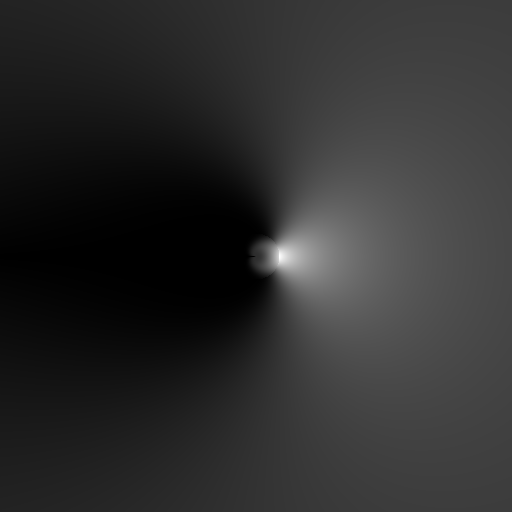
\includegraphics[scale=0.25]{figures/mitsuyasu_dfilt_wr_sqrt2.png}
 }
 \hfill
 \subtop[$U_{10}=\sqrt{8}$]
 {
 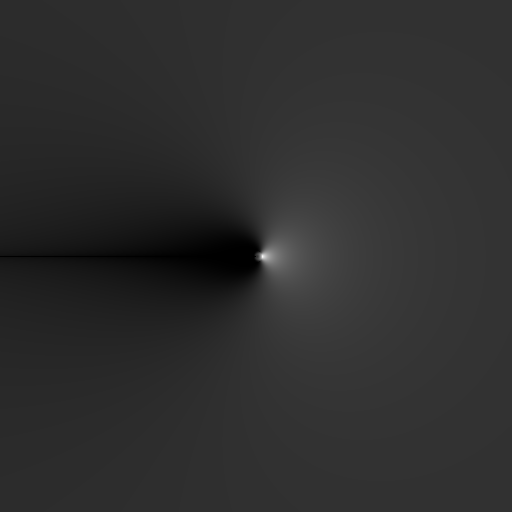
\includegraphics[scale=0.25]{figures/mitsuyasu_dfilt_wr_sqrt8.png}
 }
 \hfill
 \subtop[$U_{10}=\sqrt{50}$]
 {
 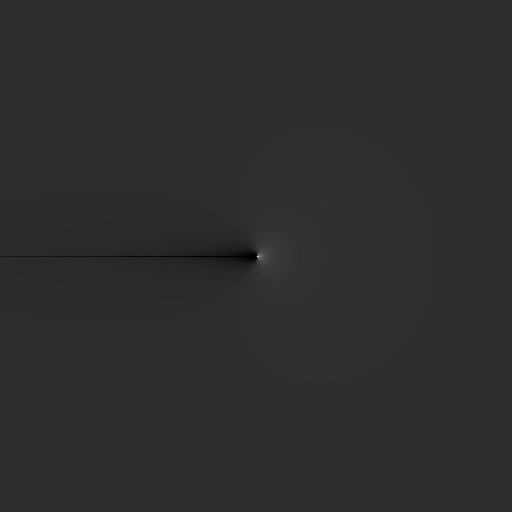
\includegraphics[scale=0.25]{figures/mitsuyasu_dfilt_wr_sqrt50.png}
 }
 \hfill
 \subtop[$U_{10}=\sqrt{200}$]
 {
 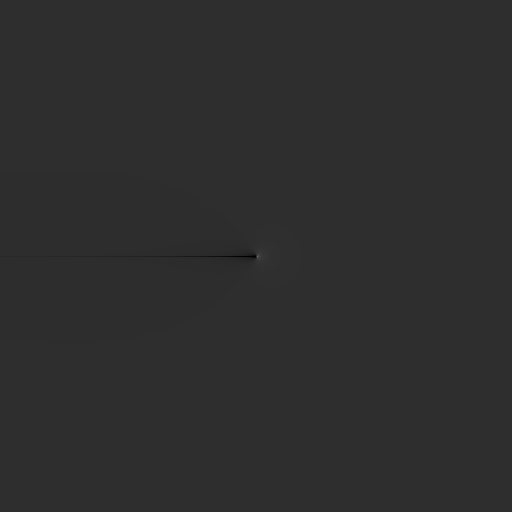
\includegraphics[scale=0.25]{figures/mitsuyasu_dfilt_wr_sqrt200.png}
 }
 \subtop
 {
 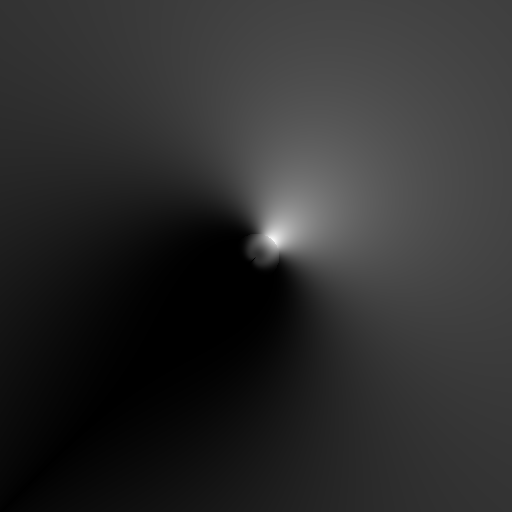
\includegraphics[scale=0.25]{figures/mitsuyasu_dfilt_wur_sqrt2.png}
 }
 \hfill
 \subtop
 {
 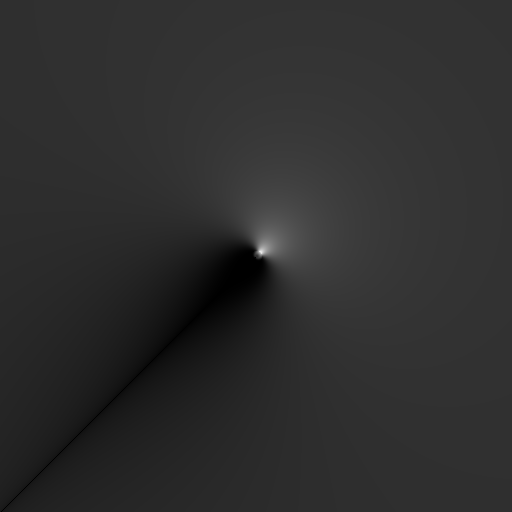
\includegraphics[scale=0.25]{figures/mitsuyasu_dfilt_wur_sqrt8.png}
 }
 \hfill
 \subtop
 {
 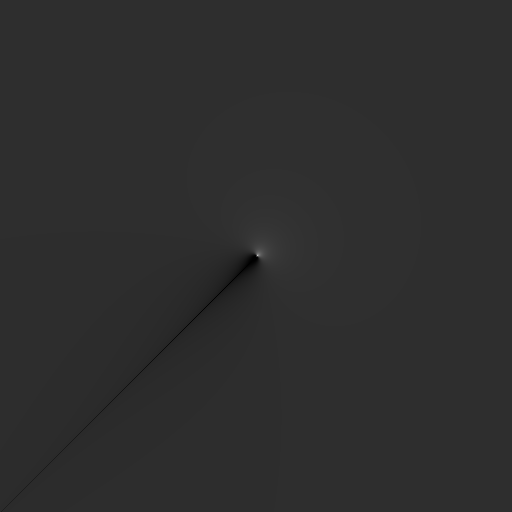
\includegraphics[scale=0.25]{figures/mitsuyasu_dfilt_wur_sqrt50.png}
 }
 \hfill
 \subtop
 {
 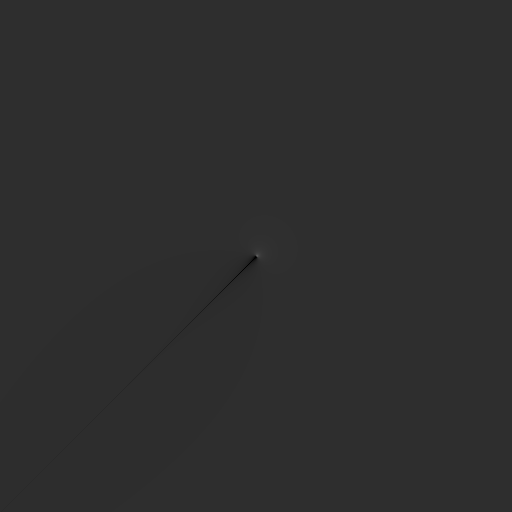
\includegraphics[scale=0.25]{figures/mitsuyasu_dfilt_wur_sqrt200.png}
 }
\caption{A set of example instances of the directional spreading function
introduced in \citet{article:Mitsuyasu1975} and extended by
\citet{article:Hasselmann1980}.
Each column corresponds to a different wind speed, starting with the weakest
one at the left. In the top row, the wind direction points to the right, in the
bottom row to the upper right.}
\label{fig:directional_filter}
\end{figure}
%
Literature provides us with a large set of different directional spreading
functions to choose from~\citep{book:windgeneratedoceanwaves}. We picked a
\emph{Cosine-2s} variant based on the work of \citet{article:Mitsuyasu1975} and 
\citet{article:Hasselmann1980}. Expressed in terms of angular frequency 
$\omega$ it is defined as follows:
\begin{equation}
\label{eq:directional_spread_mitsuyasu}
 D(\omega, \theta) =
\frac{2^{2s-1}}{\pi}~\frac{\Gamma^2(s+1)}{\Gamma(2s+1)}
~\left|\cos\left(\frac{\theta-\theta_{p}}{2}\right)\right|^{2s}
\end{equation}
with
\begin{align*}
\frac{s}{s_p} &= \begin{cases}
(\frac{\omega}{\omega_p})^{-2.5} & \omega \geq \omega_p\\
(\frac{\omega}{\omega_p})^{5} & \omega < \omega_p\\
\end{cases}
\intertext{where, according to \cite{article:Hasselmann1980}}
s_p &= \begin{cases}
9.77 & \omega \geq \omega_p\\
6.97 & \omega < \omega_p\\
\end{cases}
\end{align*}
$\Gamma$ is the \emph{gamma function}, $s$ is called the~\emph{spreading 
factor}, $\omega_p$ represents the angular frequency the frequency spectrum has 
its peak at, and $\theta_p$ is the direction of the waves at said peak. It is 
assumed that $\theta_p$ is equal the wind direction. Figure
\ref{fig:directional_filter} depicts example instances of Equation
\ref{eq:directional_spread_mitsuyasu}.
%
\subsection{Integral Domain Conversion}
%
Recall that we transform from the  \wavenumber domain to the spatial 
one. Thus, as a prerequisite, we are in need of a two-dimensional \wavenumber 
spectrum $\Theta(\mvec{k})$, but 
Equation~\ref{eq:directional_frequency_spectrum} 
gives us a directional frequency spectrum $\Theta(\omega,\theta)$. We will 
convert one spectrum form to the other according to the change of variables
theorem, with the deep water dispersion relation $\omega^2=gk$
serving as a link between angular frequency $\omega$ and \wavenumber $k$. To 
avoid possible confusion we will add subscripts to each occurence of $\Theta$ 
in order to explicitely show the parameters it takes as input.
As a first step we may transform the one dimensional frequency spectrum 
$\Theta_{\omega}(\omega)$ to the one dimensional \wavenumber 
spectrum $\Theta_k(k)$ as follows:
\begin{equation*}
 \int\Theta_k(k)~\mathrm{d}k = \int\Theta_{\omega}(\omega)~\mathrm{d}\omega\\ = 
\int\Theta_{\omega}(\omega(k))\frac{\mathrm{d}\omega}{\mathrm{d}k}~\mathrm{d}k
= \int\Theta_{\omega}(\sqrt{gk})\frac{1}{2}\sqrt{\frac{g}{k}}~\mathrm{d}k
\end{equation*}
which gives us
\begin{equation}
\label{eq:theta_k}
 \Theta_k(k) = \Theta_{\omega}(\sqrt{gk})\frac{1}{2}\sqrt{\frac{g}{k}}
\end{equation}

%
% \begin{figure}
% \centering
% \begin{tikzpicture}
% \begin{groupplot}[
% 	group style={
% 		columns=2,
% 		xlabels at=edge bottom,
% 		ylabels at=edge left,
% 		group name=plots,
% 	},
%     xlabel={\Wavenumber $k$~($\text{rad}\cdot\text{m}^{-1}$)},
%     ylabel={Energy~$\Theta$~($\text{m}^3\cdot\text{rad}^{-1}$)},
% %     legend columns=-1,
% 	width=0.5\textwidth,
% 	]
% \nextgroupplot[
%     legend style={draw=none},
%     every axis legend/.append style={nodes={right}},
% 	restrict x to domain=0:0.1,
% 	scaled ticks=false,
% 	xtick = {0,0.05,0.1},
% 	xticklabel style={/pgf/number format/fixed},
% 	]
% \addplot[
%     color=red,
%     solid,
% 	]
%     table [col sep=comma]{figures/pm_10_k.dat};
% 	\addlegendentry{$10.0~\text{m}\cdot\text{s}^{-1}$}
% \addplot[
%     color=green,
%     solid,
% 	]
%     table [col sep=comma]{figures/pm_12_k.dat};
% 	\addlegendentry{$12.5~\text{m}\cdot\text{s}^{-1}$}
% \addplot[
%     color=magenta,
%     solid,
% 	]
%     table [col sep=comma]{figures/pm_15_k.dat};
% 	\addlegendentry{$15.0~\text{m}\cdot\text{s}^{-1}$}
% \addplot[
%     color=black,
%     solid,
% 	]
%     table [col sep=comma]{figures/pm_17_k.dat};
% 	\addlegendentry{$17.5~\text{m}\cdot\text{s}^{-1}$}
% \addplot[
%     color=blue,
%     solid,
% 	]
%     table [col sep=comma]{figures/pm_20_k.dat};
% 	\addlegendentry{$20.0~\text{m}\cdot\text{s}^{-1}$}
% \nextgroupplot[
%     legend style={draw=none},
%     every axis legend/.append style={nodes={right}},
% 	restrict x to domain=0:0.5,
% 	xtick = {0,0.25,0.5},
% 	xticklabel style={/pgf/number format/fixed},
% ]
% \addplot[
%     color=blue,
%     solid,
%     ]
%     table [col sep=comma]{figures/pm_10_k.dat};
% \addlegendentry{PM}
% \addplot[
%     color=red,
%     solid,
%     ]
%     table [col sep=comma]{figures/j_10_10km_k.dat};
% \addlegendentry{10 km}
% \addplot[
%     color=green,
%     solid,
%     ]
%     table [col sep=comma]{figures/j_10_25km_k.dat};
% \addlegendentry{25 km}
% \addplot[
%     color=magenta,
%     solid,
%     ]
%     table [col sep=comma]{figures/j_10_50km_k.dat};
% \addlegendentry{50 km}
% \addplot[
%     color=black,
%     solid,
%     ]
%     table [col sep=comma]{figures/j_10_75km_k.dat};
% \addlegendentry{75 km}
% \end{groupplot}
% \end{tikzpicture}
% \caption{One dimensional frequency spectra $\Theta_{\omega}(\omega$) converted
% into one dimensional \wavenumber spectra $\Theta_k(k)$. Left: The Pierson 
% Moskowitz spectra from Figure~\ref{fig:pm_spectra}(a). Right: The JONSWAP 
% spectra from Figure~\ref{fig:jonswap_spectra}(a).}
% \label{fig:jonswap_spectra_fetches_k}
% \end{figure}
%
% A set of one dimensional wave spectra $\Theta_k(k)$ may be seen in
% Figure~\ref{fig:jonswap_spectra_fetches_k}. Note the difference in scale on the ordinate
% in comparison to the one dimensional frequency spectra $\Theta_{\omega}(\omega)$
% depicted in Figure~\ref{fig:pm_spectra} and Figure~\ref{fig:jonswap_spectra}.
%
\begin{figure}
\centering
\subbottom
{
\label{sfig:polar}
\begin{tikzpicture}
\begin{axis}[
    width=0.5\paperwidth,
    view={-20}{30},
    mesh/ordering=y varies,
    zlabel={Energy~$\Theta$~(\si{\square\meter\second})},
    xlabel={Frequency~$\omega$~(\si{\radian\per\second})},
    ylabel={Direction~$\theta$~(\si{\radian})},
    ]
\addplot3[surf,
    ]
    table [col sep=comma]{figures/jonswap_w15_f100_omega_angle.dat};
\end{axis}
\end{tikzpicture}
}
\subbottom
{
\label{sfig:wave_vector}
\begin{tikzpicture}
\begin{axis}[
    width=0.5\paperwidth,
    view={-20}{30},
    mesh/ordering=y varies,
    xtick = {0,0.1,0.2},
    zlabel={Energy~$\Theta$~(\si{\raiseto{4}\meter\per\square\radian})},
    xlabel={$k_x$~(\si{\radian\per\second})},
    ylabel={$k_z$~(\si{\radian\per\second})},
    ]
\addplot3[surf,
    ]
    table [col sep=comma]{figures/jonswap_w15_f100_kx_ky.dat};
\end{axis}
\end{tikzpicture}
}
\caption{The JONSWAP frequency spectrum with wind speed $U_{10} = \SI{15}{\meter\per\second}$
and fetch $F = \SI{100}{\km}$, located in two different domains. Top: The polar
coordinate domain $\omega \times \theta$, the wind direction points in the
direction of the positive $\omega$ axis. Bottom: The \wavevector domain
$k_x \times k_z$, the wind direction points in the direction of the positive
$k_x$ axis. Note the difference in scale between the two vertical axes.}
\label{fig:jonswap_3d_omega_theta_kx_ky}
\end{figure}
%

Given $\Theta_k(k)$, we are able to rewrite the directional frequency spectrum
$\Theta_{\omega, \theta}(\omega, \theta)$ from
Equation~\ref{eq:directional_frequency_spectrum} in terms of \wavenumber $k$:
%
\begin{equation}
\label{eq:theta_k_polar}
 \Theta_{k,\theta}(k,\theta) = \Theta_k(k)D(\sqrt{gk},\theta)
\end{equation}
%
As the last step we need to convert from polar coordinate pairs 
$(k,\theta)$ to Cartesian \wavenumber coordinates $\mvec{k}$. Said conversion 
is accomplished as follows:
%
\begin{equation}
\label{eq:theta_cart_to_polar}
\int\Theta_{\mvec{k}}(\mvec{k})~\mathrm{d}\mvec{k} = 
\int\int\Theta_{k,\theta}(k,\theta)\frac{1}{k}~\mathrm{d}\theta~\mathrm{d}k
\end{equation}
%
By combining Equations~\ref{eq:directional_frequency_spectrum}, 
~\ref{eq:theta_k} and~\ref{eq:theta_cart_to_polar} we get the two-dimensional
\wavenumber spectrum:
%
\begin{align}
\Theta_{\mvec{k}}(\mvec{k}) = \Theta_{\omega,\theta}(\sqrt{gk}, 
\theta)\frac{1}{2k}\sqrt{\frac{g}{k}} &&
\theta = \arctan\left(\frac{k_z}{k_x}\right)
\end{align}
%
An instance of a directional frequency spectrum as well as its equivalent
directional \wavenumber spectrum are depicted in Figure
\ref{fig:jonswap_3d_omega_theta_kx_ky}.

Now we are able to preserve integral equality between different representations 
of $\Theta$, as long as we use the deep water dispersion relation. One may do 
the math for another dispersion relation, given that we have laid out the path
one has to take. Still, in the context of this work, we only concern ourselves
with waves in deep water.
%
\subsection{Two-Dimensional Wave Spectra}
% \label{subsec:two_dimensional_frequency_spectra}
%
Beforehand we introduced the combination of a one dimensional 
frequency spectrum with a directional spreading function in order to generate a 
two-dimensional frequency spectrum. We have seen that there are different forms
of two-dimensional wave spectra, such as the directional frequency spectrum
$\Theta(\omega, \theta)$, the \wavenumber spectrum in polar form
$\Theta(k, \theta)$, and the \wavenumber spectrum in Cartesian form
$\Theta(\mvec{k})$. Moreover, given a dispersion relation, we 
are able to convert between all these different forms of a spectrum. Now, we 
may move on to wave spectra which have been explicitly introduced in a two 
dimensional form by oceanographic research.

\subsection{Donelan Spectrum}
%
The Donelan spectrum is a directional frequency spectrum which has 
been developed by \citet{article:Donelan1985} based on data 
collected both on Lake Ontario and at the \emph{Canadian Centre for Inland 
Waters}'s wind-wave flume. At its core, the Donelan spectrum still is a one 
dimensional frequency spectrum combined with a directional spreading function, 
but it improves upon certain key aspects compared to the models discussed 
beforehand. The most prominent of said improvements is the ability of the 
Donelan spectrum to model the transition between developing and fully developed 
seas. Other improvements include the possibility for wind direction and peak 
wave direction to differ, as well as a directional spreading function which both
matches existing data more closely and is simpler in formulation than the one 
introduced by \citet{article:Mitsuyasu1975}.

The energy given by the one dimensional Donelan frequency spectrum depends on 
the frequency itself, the position of that frequency in the spectrum 
$(\omega/\omega_p)$ and on the intensity of wind input $\Omega_c = U_c/c_p$, 
where $U_c$ is the component of the wind in the direction 
of travel of the waves at the spectral peak, and $c_p$ is the phase velocity of 
the waves at the spectral peak. The directional spreading on the other hand is 
related only to $\omega/\omega_p$.
According to \citeauthor{article:Donelan1985}, wind component $U_c$ is defined
based on wind speed $U_{10}$:
\begin{align}
 U_c = U_{10}\cos(\theta_w-\theta_p) && \abs{\theta_w-\theta_p}\leq\SI{15}{\degree}
\end{align}
where $\theta_w$ is the direction of wind speed $U_{10}$, and $\theta_p$
represents the direction of travel of the waves at the spectral peak.
We may move on to the directional Donelan frequency spectrum,
which is as follows:
\begin{equation}
\label{eq:donelan:dfreqspectrum}
 \Theta(\omega, \theta) = \frac{1}{2}\Theta(\omega)\beta\sech^2
\{\beta[\theta - \theta_p]\}
\end{equation}
From the equation one may see that the directional spread is the following:
\begin{equation}
\label{eq:donelan:dspread}
  D(\omega, \theta) = \frac{1}{2}\beta\sech^2\{\beta[\theta - \theta_p]\}
\end{equation}
where $\sech$ is the \emph{hyperbolic secant function}.
The width of the directional spread is determined by the
parameter $\beta$, which is defined as:
\begin{align}
\label{eq:donelan:beta}
\beta &= \begin{cases}
	2.61(\omega/\omega_p)^{1.3} & 0.56 < \omega/\omega_p < 0.95\\
	2.28(\omega/\omega_p)^{-1.3} & 0.95 \leq \omega/\omega_p < 1.6\\
	1.24 & \text{otherwise}
    \end{cases}
\end{align}
Given wind input $U_c$, and the inverse wave age $\Omega_c$ based on the
component of the wind in the direction of the peak waves, then, assuming deep
water, we may write peak angular frequency $\omega_p$ in step with
Equation~\ref{eq:inverse_wave_age_deep_water}:
\begin{equation}
 \omega_{p} = \Omega_c\frac{g}{U_{c}}
\end{equation}
\citeauthor{article:Donelan1985} defines inverse wave age $\Omega_c$ based on
dimensionless fetch $\chi$ as follows:
\begin{align}
\label{eq:donelan:omegac}
 \Omega_c = 11.6\chi^{-0.23} && \chi = \frac{gF}{U_{c}^{2}}
\end{align}
where the inverse wave age is restricted to
the interval ${\Omega_c\in\interval[open left, open right]{0.83}{5}}$,
and $F$ denotes the fetch in meters.
The Donelan directional spreading function from Equation~\ref{eq:donelan:dspread}
does not only differ in form from the one proposed by
\citet{article:Mitsuyasu1975} and \citet{article:Hasselmann1980},
but also in sensitivity, or rather insensitivity, to wind speed, see
Figure~\ref{fig:donelan_directional_filter}. That is because the Donelan
formulation in Equation~\ref{eq:donelan:beta} employs the ratio
$\omega/\omega_p$ whereas
\citeauthor{article:Mitsuyasu1975} and \citeauthor{article:Hasselmann1980}
use comparisons with absolute values.

With the directional spread covered, we move on to the one dimensional frequency
spectrum as described by \cite{article:Donelan1985}. We may write:
\begin{equation}
 \Theta(\omega) = 
\alpha g^2 \omega^{-5}(\omega/\omega_p) \exp\left[-\left(\frac{\omega_p}{\omega}
\right)^4\right]\gamma^r
\end{equation}
with
\begin{align*}
\gamma &= \begin{cases}
	1.7 & 0.83 < \Omega_c < 1\\
	1.7 + 6.0\lg(\Omega_c) & 1\leq\Omega_c < 5
	\end{cases}\\
r &= \exp\left[-\frac{\left(\omega -
\omega_p\right)^2}{2\sigma^2\omega_p^2}\right] \\
\sigma &= 0.08\left(1 + \frac{4}{\Omega_c^3}\right)\\
\alpha &= 0.006~\Omega_c^{0.55}
\end{align*}
% where $F$ denotes the fetch in meters, and $\chi$ represents the dimensionless
% fetch.
% $U_{c}$ denotes the wind speed in 
% meters per second at a height of ten meters above the sea surface.
where, in lockstep with the JONSWAP spectrum, 
$\gamma^r$ is called the peak enhancement factor, $\sigma$ the peak width 
parameter, and $\alpha$ the equilibrium range parameter.
% Moreover, $\Omega_c$ denotes the inverse 
% wave age based on the component of the wind in the direction of the peak waves,
% and is restricted to the interval $\Omega_c \in \interval[open left, open 
% right]{0.83}{5}$.
%
\begin{figure}[p]
 \centering
 \subtop[][$U_{c}=\sqrt{2}$]
 {
 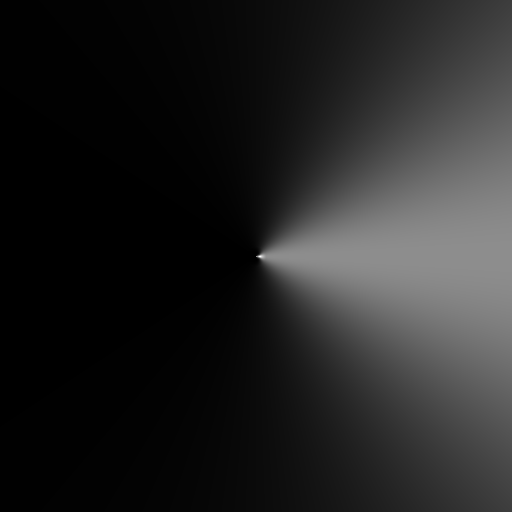
\includegraphics[scale=0.25]{figures/donelan_dfilt_wr_sqrt2.png}
 }
 \hfill
 \subtop[$U_{c}=\sqrt{8}$]
 {
 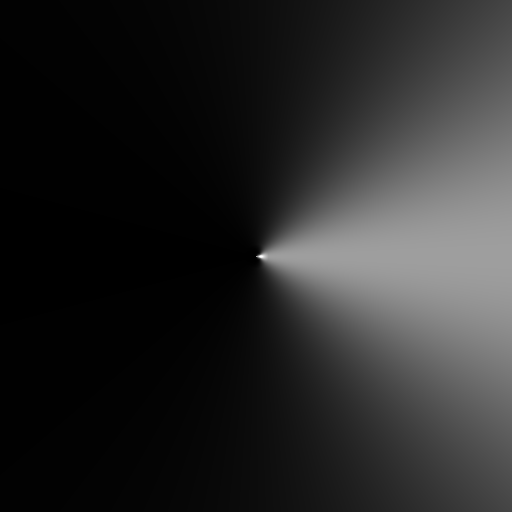
\includegraphics[scale=0.25]{figures/donelan_dfilt_wr_sqrt8.png}
 }
 \hfill
 \subtop[$U_{c}=\sqrt{50}$]
 {
 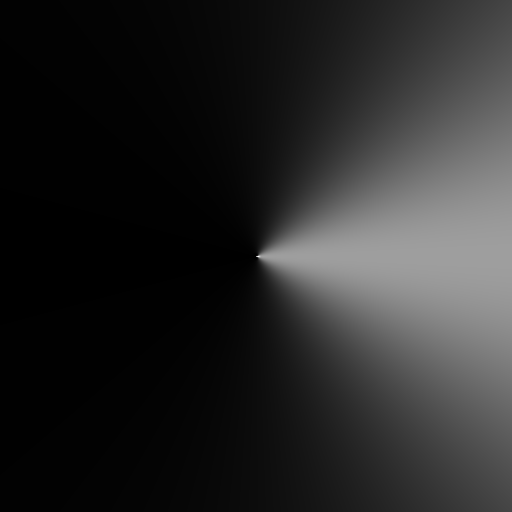
\includegraphics[scale=0.25]{figures/donelan_dfilt_wr_sqrt50.png}
 }
 \hfill
 \subtop[$U_{c}=\sqrt{200}$]
 {
 
\includegraphics[scale=0.25]{figures/donelan_dfilt_wr_sqrt200.png}
 }
 \subtop
 {
 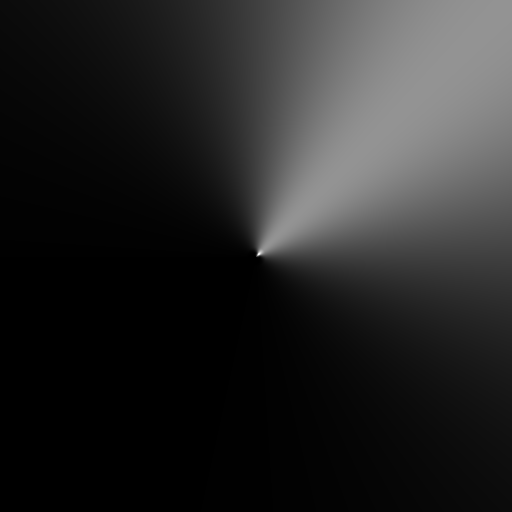
\includegraphics[scale=0.25]{figures/donelan_dfilt_wur_sqrt2.png}
 }
 \hfill
 \subtop
 {
 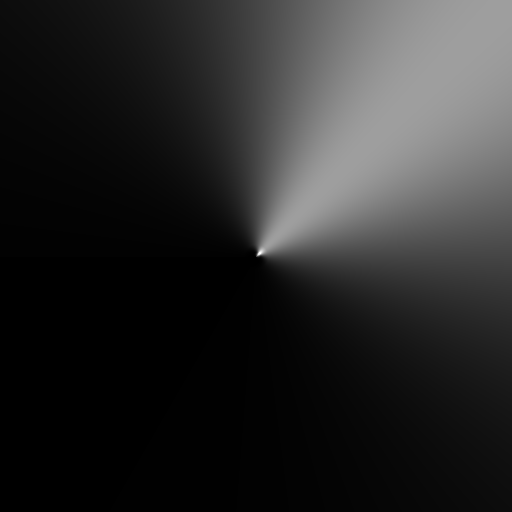
\includegraphics[scale=0.25]{figures/donelan_dfilt_wur_sqrt8.png}
 }
 \hfill
 \subtop
 {
 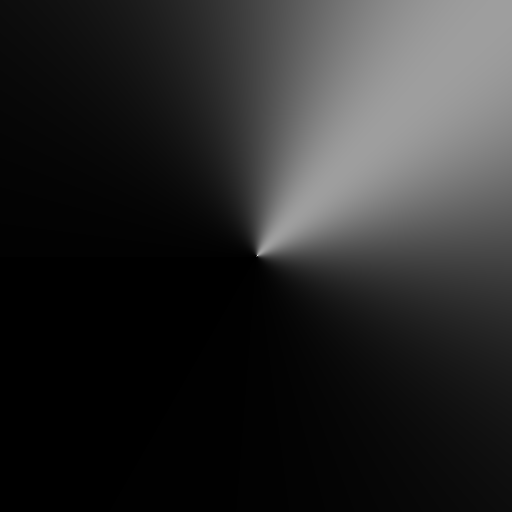
\includegraphics[scale=0.25]{figures/donelan_dfilt_wur_sqrt50.png}
 }
 \hfill
 \subtop
 {
 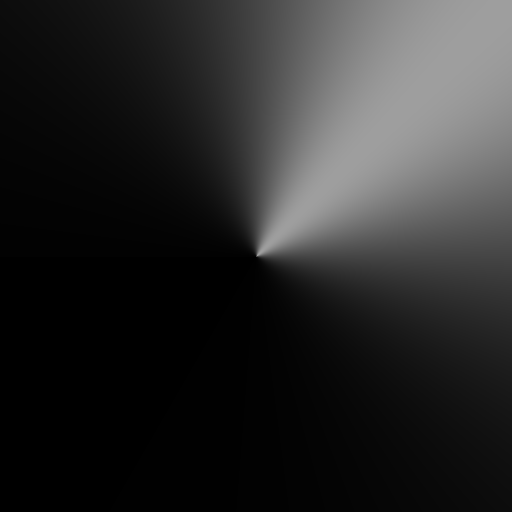
\includegraphics[scale=0.25]{figures/donelan_dfilt_wur_sqrt200.png}
 }
\caption{A set of instances of the directional spreading function intoduced by
\citet{article:Donelan1985}. Each column 
corresponds to a different wind speed, starting with the weakest one at the 
left. In the top row, the wind direction points to the right, in the bottom row 
to the upper right. 
One can see that the directional spread changes only slightly in intensity and
form with increasing wind speed $U_{c}$.}
\label{fig:donelan_directional_filter}
\end{figure}
%
%\begin{figure}
 %\centering
 %\subtop[][$U_{c}=\sqrt{2}$]
 %{
 %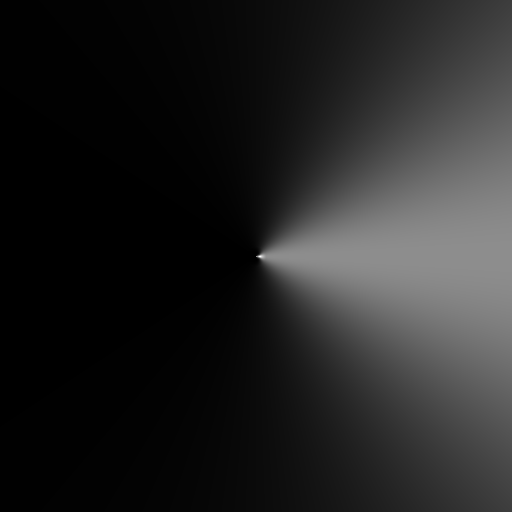
\includegraphics[scale=0.25]{figures/donelan_dfilt_wr_sqrt2.png}
 %}
 %\hfill
 %\subtop[][$U_{c}=\sqrt{8}$]
 %{
 %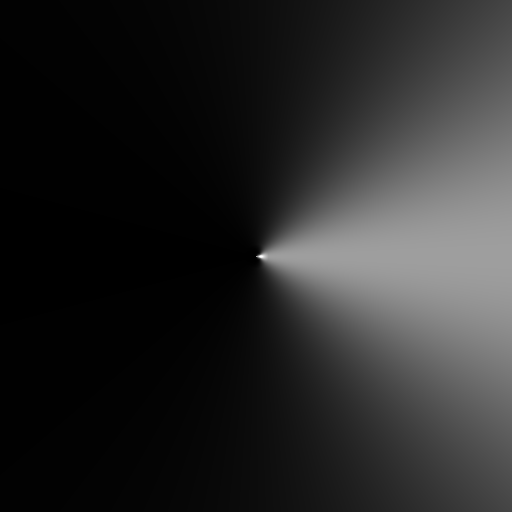
\includegraphics[scale=0.25]{figures/donelan_dfilt_wr_sqrt8.png}
 %}
 %\hfill
 %\subtop[][$U_{c}=\sqrt{50}$]
 %{
 %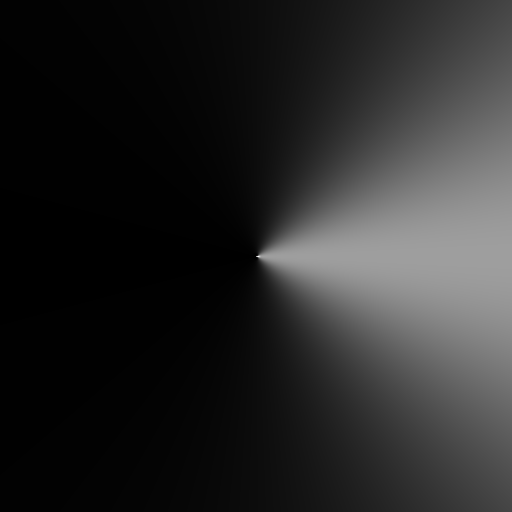
\includegraphics[scale=0.25]{figures/donelan_dfilt_wr_sqrt50.png}
 %}
 %\hfill
 %\subtop[][$U_{c}=\sqrt{200}$]
 %{
 %
\includegraphics[scale=0.25]{figures/donelan_dfilt_wr_sqrt200.png}
 %}
 %%\hfill
 %%\subtop[][$U_{10}=\sqrt{2}$]
 %%{
 %%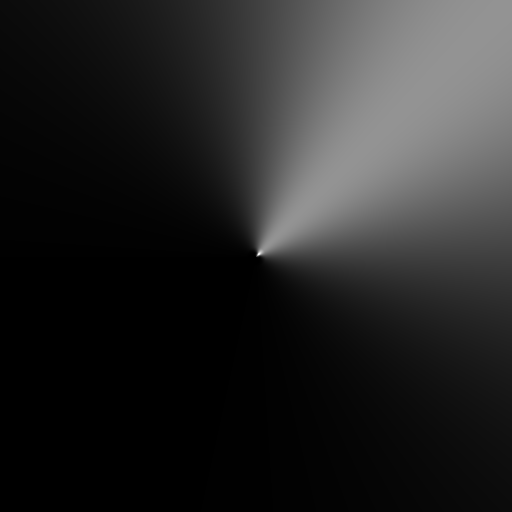
\includegraphics[scale=0.115]{figures/donelan_dfilt_wur_sqrt2.png}
 %%}
 %%\hfill
 %%\subtop[][$U_{10}=\sqrt{8}$]
 %%{
 %%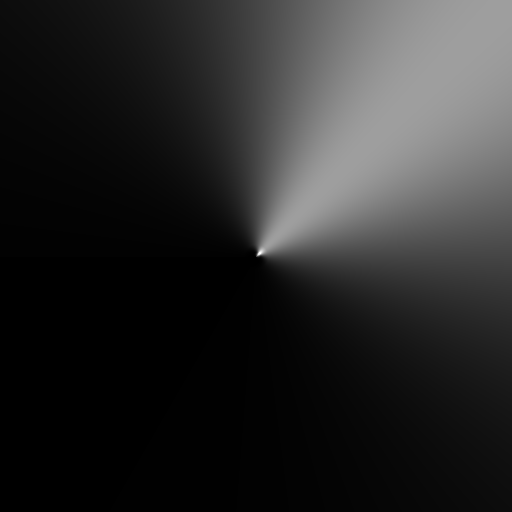
\includegraphics[scale=0.115]{figures/donelan_dfilt_wur_sqrt8.png}
 %%}
 %%\hfill
 %%\subtop[][$U_{10}=\sqrt{50}$]
 %%{
 %%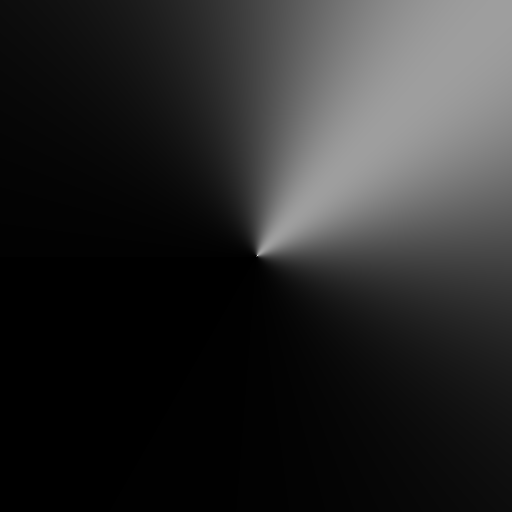
\includegraphics[scale=0.115]{figures/donelan_dfilt_wur_sqrt50.png}
 %%}
 %%\hfill
 %%\subtop[][$U_{10}=\sqrt{200}$]
 %%{
 %%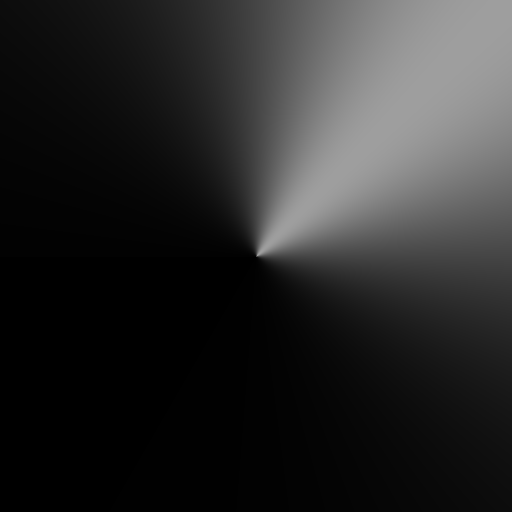
\includegraphics[scale=0.115]{figures/donelan_dfilt_wur_sqrt200.png}
 %%}
 %\subtop[$U_{10}=\sqrt{2}$]
 %{
 %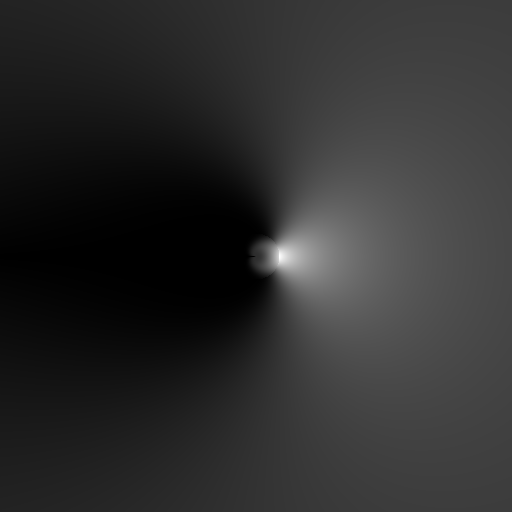
\includegraphics[scale=0.25]{figures/mitsuyasu_dfilt_wr_sqrt2.png}
 %}
 %\hfill
 %\subtop[$U_{10}=\sqrt{8}$]
 %{
 %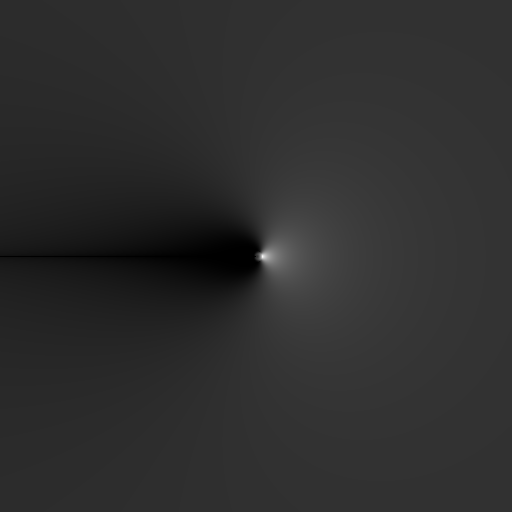
\includegraphics[scale=0.25]{figures/mitsuyasu_dfilt_wr_sqrt8.png}
 %}
 %\hfill
 %\subtop[$U_{10}=\sqrt{50}$]
 %{
 %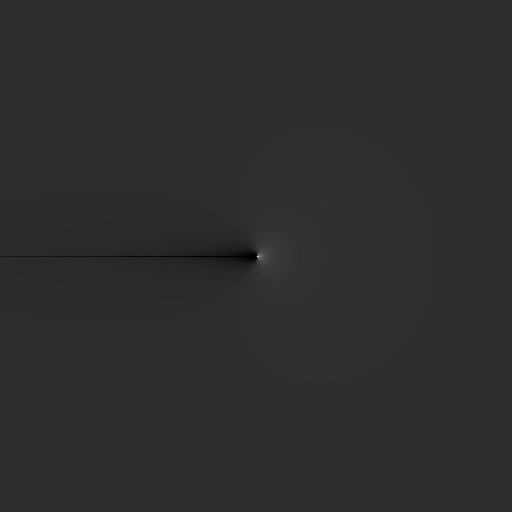
\includegraphics[scale=0.25]{figures/mitsuyasu_dfilt_wr_sqrt50.png}
 %}
 %\hfill
 %\subtop[$U_{10}=\sqrt{200}$]
 %{
 %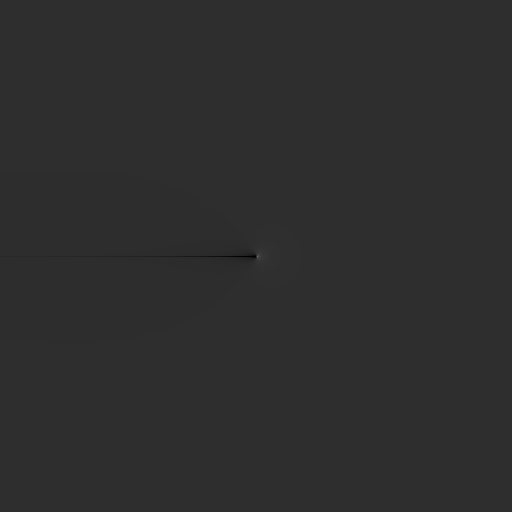
\includegraphics[scale=0.25]{figures/mitsuyasu_dfilt_wr_sqrt200.png}
 %}
 %%\hfill
 %%\subtop
 %%{
 %%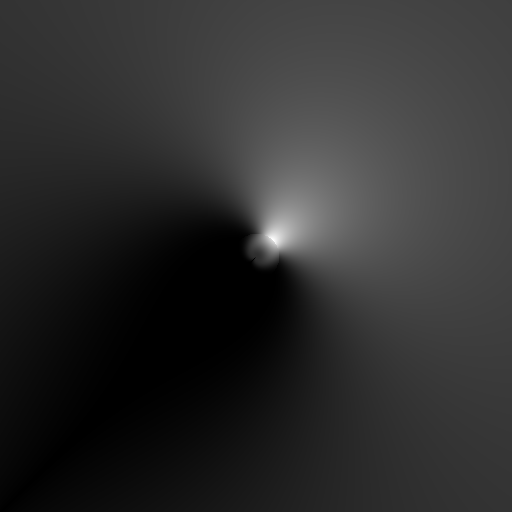
\includegraphics[scale=0.115]{figures/dfilt_wur_sqrt2.png}
 %%}
 %%\hfill
 %%\subtop
 %%{
 %%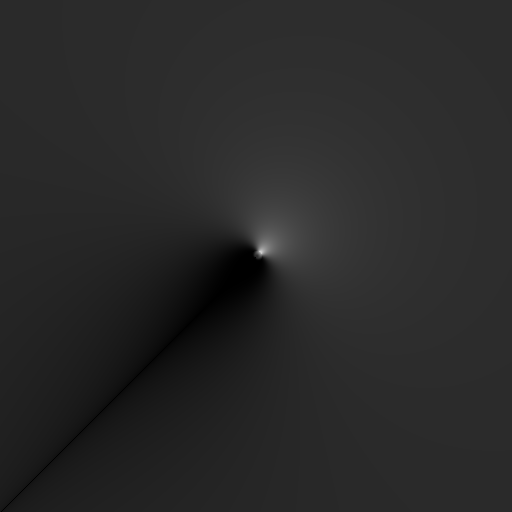
\includegraphics[scale=0.115]{figures/dfilt_wur_sqrt8.png}
 %%}
 %%\hfill
 %%\subtop
 %%{
 %%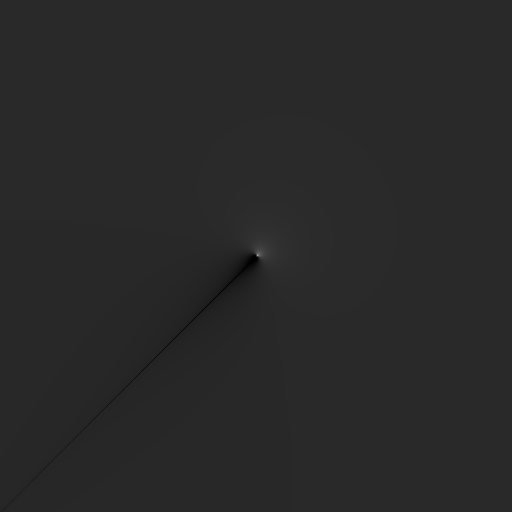
\includegraphics[scale=0.115]{figures/dfilt_wur_sqrt50.png}
 %%}
 %%\hfill
 %%\subtop
 %%{
 %%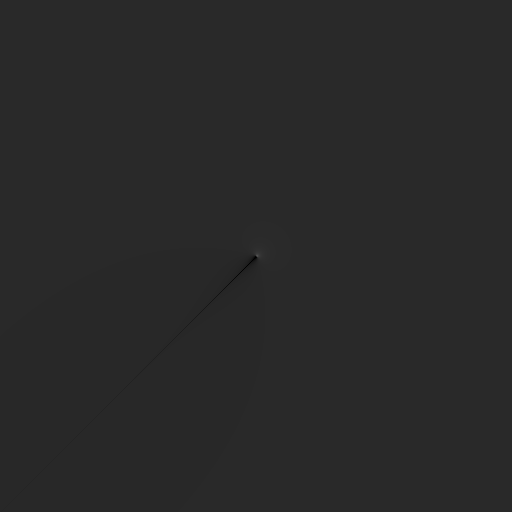
\includegraphics[scale=0.115]{figures/dfilt_wur_sqrt200.png}
 %%}
%\caption{Comparison between~\citet{article:Donelan1985} directional spread
%(top row) and the one proposed by~\citet{article:Mitsuyasu1975} and
%\citet{article:Hasselmann1980} (bottom row). Both sets were generated with
%identical input data.
%%In contrast to the directional spread displayed in the bottom row,
%One can see that the directional spread by \citeauthor{article:Donelan1985}
%changes only slightly in intensity and form with increasing wind speed.
%The directional spread by \citeauthor{article:Mitsuyasu1975} and
%\citeauthor{article:Hasselmann1980}, on the other hand, undergoes severe
%alterations in form and intensity.}
%\label{fig:directional_filter_comp}
%\end{figure}
%
%
\begin{figure}[p]
\centering
\begin{tikzpicture}
\begin{groupplot}[
	group style={
		columns=2,
		xlabels at=edge bottom,
		ylabels at=edge left,
	},
    xlabel={Frequency~$\omega$~(\si{\radian\per\second})},
    ylabel={Energy~$\Theta$~(\si{\square\meter\second})},
	width=0.5\textwidth,
	scaled ticks=false,
	]
\nextgroupplot[
%	title={(a)},
    legend style={draw=none},
    every axis legend/.append style={nodes={right}},
	restrict x to domain=0.25:3,
	]
\addplot[
    color=blue,
    solid,
    ]
    table [col sep=comma]{figures/d_pm_10.dat};
\addlegendentry{PM}
\addplot[
    color=red,
    solid,
    ]
    table [col sep=comma]{figures/d_10_750km.dat};
\addlegendentry{\SI{750}{\km}}
\addplot[
    color=black,
    solid,
    ]
    table [col sep=comma]{figures/d_10_500km.dat};
\addlegendentry{\SI{500}{\km}}
\addplot[
    color=magenta,
    solid,
    ]
    table [col sep=comma]{figures/d_10_250km.dat};
\addlegendentry{\SI{250}{\km}}
\addplot[
    color=green,
    solid,
    ]
    table [col sep=comma]{figures/d_10_100km.dat};
\addlegendentry{\SI{100}{\km}}
%\addplot[
    %color=red,
    %solid,
    %]
    %table [col sep=comma]{figures/d_10_50km.dat};
%\addlegendentry{50 km}
\nextgroupplot[
	%title={(b)},
    legend style={draw=none},
    every axis legend/.append style={nodes={right}},
	xtick = {0,2.5,5},
	yticklabel style={/pgf/number format/fixed},
	restrict x to domain=1.8:5,
]
\addplot[
    color=blue,
    solid,
	]
    table [col sep=comma]{figures/d_pm_wp_25.dat};
\addlegendentry{PM}
\addplot[
    color=green,
    solid,
	]
    table [col sep=comma]{figures/d_j_wp_25_wc_083.dat};
\addlegendentry{JONSWAP $0.83$}
\addplot[
    color=magenta,
    solid,
	]
    table [col sep=comma]{figures/d_j_wp_25_wc_4.dat};
\addlegendentry{JONSWAP $4$}
\addplot[
    color=red,
    solid,
	]
    table [col sep=comma]{figures/d_wp_25_wc_083.dat};
\addlegendentry{Donelan $0.83$}
\addplot[
    color=black,
    solid,
	]
    table [col sep=comma]{figures/d_wp_25_wc_4.dat};
\addlegendentry{Donelan $4$}
\end{groupplot}
\end{tikzpicture}
\caption{Left: Donelan frequency spectra with different fetch values $F$, 
Pierson Moskowitz spectrum for comparison ($U_{10} = \SI{10}{\meter\per\second}$). The
Donelan spectrum converges towards the Pierson Moskowitz spectrum with
increasing fetch, but overshoots.
Right: 
JONSWAP and Donelan spectra with different inverse wave age values $\Omega_c$, 
Pierson Moskowitz spectrum for comparison ($\omega_p = 2.5$).
Given specific values for $\Omega_c$, the Donelan spectrum transitions well
between a developing and a fully developed sea.}
\label{fig:donelan_spectra}
\end{figure}
%
In contrast to the JONSWAP spectrum introduced earlier, the one dimensional 
frequency spectrum as given by \citeauthor{article:Donelan1985} is able to
transition to fully developed state. As one can see in
Figure~\ref{fig:donelan_spectra}, said transition does work if inverse wave age
$\Omega_c$ is given explicitely, instead of being estimated based on fetch.
We may conclude that Equation~\ref{eq:donelan:omegac} is not that good an
approximation of inverse wave age $\Omega_c$, especially because it does not
ensure a lower limit of ${\Omega_c=0.83}$ for large fetch.
%
\subsection{Unified Spectrum}
\label{sec:unified_spectrum}
%
The Unified spectrum is a directional \wavenumber spectrum introduced by
\citet{article:Elfouhaily1997}. It consists of a one 
dimensional \wavenumber spectrum combined with a directional spreading 
function. All of the spectral models which we introduced beforehand focus on 
the \emph{long-wave regime}, which, according to \citeauthor{article:Elfouhaily1997},
is defined as the \wavenumber range $k < 10\times k_p$, where $k_p$ is
the \wavenumber the spectrum has its peak at. The Unified spectrum on the
other hand models the~\emph{entire} \wavenumber range, including the
\emph{short-wave regime}, which is defined as $k >= 10\times k_p$.
Because the short-wave regime extends into the gravity-capillary wave domain,
we need a dispersion relation which extends into said domain too.
We may write:
\begin{align*}
\omega^2 = gk\left[1 + \left(\frac{k}{k_m}\right)^2\right] &&
k_m = \sqrt{\frac{p_w g}{T}} = \SI{370}{\radian\per\meter}
\end{align*}
where $k_m$ is the \wavenumber at which gravity-capillary waves on an air-water
interface have their minimum phase velocity~\citep{lamb:1945}.
The constants $p_w$, $g$ and $T$ are water density, acceleration due to
earth's gravity, and water surface tension, respectively.

The combined works of \citet{article:Hasselman1973}, \citet{article:Mitsuyasu1975}
and \citet{article:Donelan1985} serve as foundation for the Unified spectrum. 
Moreover, \citeauthor{article:Elfouhaily1997} did expand their model to the
short-wave regime by incorporating related theory \citep{book:Kitaigorodskii1970,
article:Phillips1985} and observations \citep{article:CoxMunk1954,article:Jaehne1990a,
article:Hara1994}. We may write the Unified spectrum as follows:
%
\begin{equation}
\label{eq:unified:theta}
 \Theta(k, \theta) = \frac{1}{2\pi}\Theta(k)\{1 + \Delta(k) + \cos[2(\theta - \theta_p)]\}
\end{equation}
%
where $\theta_p$ is the direction of travel of the waves at the spectral peak. 
Since the Unified spectrum is given in terms of \wavenumber, we are in need of a 
\wavenumber-based formulation of its foundation, namely the Pierson Moskowitz 
spectrum \citep{article:PiersonMoskowitz1964}, as well as the peak enhancement
factor introduced by \citet{article:Hasselman1973}.
\citeauthor{article:Elfouhaily1997} give the \wavenumber formulation of the
Pierson Moskowitz spectrum as follows:
%
\begin{equation*}
 L_{PM}(k) = \exp\left[-\frac{5}{4} \left(\frac{k_p}{k}\right)^2 \right]
\end{equation*}
where $k_p$ denotes the \wavenumber the spectrum has its peak at.
According to \citeauthor{article:Elfouhaily1997} it is defined as:
\begin{align*}
%\label{eq:unified:k_p}
k_p &= g\frac{\Omega_c^2}{U_{10}^2}
\end{align*}
where $U_{10}$ represents the wind speed in meters per second at a height of ten
meters above the sea surface, and $\Omega_c$ denotes the inverse wave age based
on the component of the wind in the direction of the peak waves.
The latter term is given by \citeauthor{article:Elfouhaily1997} as follows:
\begin{align}
\label{eq:unified:omega_c} \Omega_c = 0.84 \tanh\left[\left(\frac{\chi}{\chi_0}\right)^{0.4}\right]^{-0.75} && \chi_0 = 2.2 \times 10^4
\end{align}
where $\chi$ is the dimensionless fetch. For simplicity's sake we will replicate
the definition of dimensionless fetch $\chi$ from before:
\begin{align*}
 \chi &= \frac{gF}{U_{10}^{2}}
\end{align*}
with $F$ representing the dimensional fetch in meters.
%In lockstep with the JONSWAP spectrum, $\gamma^r$ is 
%called the peak enhancement factor and $\sigma$ represents the peak width 
%parameter.
According to \citeauthor{article:Elfouhaily1997}, the inverse wave age
should be restricted to the range $\Omega_c \in \interval[open right]{0.84}{5}$.
From Equation~\ref{eq:unified:omega_c} one may see that $\Omega_c$ is guaranteed
a lower limit of $0.84$ for large fetch e.g. fully developed seas.
It follows that the Unified spectrum is not prone to overdevelopment with
increasining fetch, which is a notable improvement 
compared to the spectral models of \citet{article:Hasselman1973}
and \citet{article:Donelan1985} (Figure~\ref{fig:unified_spectra}).

\citeauthor{article:Elfouhaily1997} give the \wavenumber formulation of the
peak enhancement factor as follows:
\begin{equation*}
J_p = \gamma^{\Gamma}
\end{equation*}
where base $\gamma$ depends only on inverse wave age $\Omega_c$, and exponent
$\Gamma$ requires peak \wavenumber $k_p$ and the peak width parameter $\sigma$.
We may write:
\begin{align*}
\gamma &= \begin{cases}
	1.7 & 0.84 \leq \Omega_c < 1 \\
	1.7 + 6.0\lg(\Omega_c) & 1\leq\Omega_c < 5
	\end{cases} \\
\Gamma &= \exp\left[-\frac{\left(\sqrt{\frac{k}{k_p}}-1\right)^2}{2\sigma^2}\right] \\
\sigma &= 0.08\left(1 + \frac{4}{\Omega_c^3}\right)
\end{align*}
%
\begin{figure}
\centering
%\tikzset{external/force remake}
\begin{tikzpicture}
\begin{groupplot}[
	group style={
		rows=1,
		columns=2,
		xlabels at=edge bottom,
		ylabels at=edge left,
	},
    xlabel={\Wavenumber~$k$~(\si{\radian\per\meter})},
    ylabel={Energy~$\Theta$~(\si{\cubic\meter\per\radian})},
	width=0.5\textwidth,
	scaled ticks=false,
	]
\nextgroupplot[
    legend style={draw=none},
    every axis legend/.append style={nodes={right}},
	restrict x to domain=0:0.4,
	]
\addplot[
    color=blue,
    solid,
    ]
    table [col sep=comma]{figures/pm_10_k.dat};
\addlegendentry{PM}
\addplot[
    color=red,
    solid,
    ]
    table [col sep=comma]{figures/u_10_750km_k.dat};
\addlegendentry{\SI{750}{\km}}
\addplot[
    color=black,
    solid,
    ]
    table [col sep=comma]{figures/u_10_500km_k.dat};
\addlegendentry{\SI{500}{\km}}
\addplot[
    color=magenta,
    solid,
    ]
    table [col sep=comma]{figures/u_10_250km_k.dat};
\addlegendentry{\SI{250}{\km}}
\addplot[
    color=green,
    solid,
    ]
    table [col sep=comma]{figures/u_10_100km_k.dat};
\addlegendentry{\SI{100}{\km}}
%\addplot[
    %color=red,
    %solid,
    %]
    %table [col sep=comma]{figures/u_10_50km_k.dat};
%\addlegendentry{50 km}
\nextgroupplot[
    legend style={draw=none},
    every axis legend/.append style={nodes={right}},
	xticklabel style={
		/pgf/number format/fixed,
	},
	xmin = 0,
	xmax = 0.2,
	ymax = 15,
	enlarge x limits = true,
	]
\addplot[
    color=blue,
    solid,
    ]
    table [col sep=comma]{figures/pm_10_k.dat};
\addlegendentry{PM}
\addplot[
    color=red,
    solid,
    ]
    table [col sep=comma]{figures/j_10_1000km_k.dat};
\addlegendentry{JONSWAP}
\addplot[
    color=red,
    solid,
	forget plot,
    ]
    table [col sep=comma]{figures/j_10_1500km_k.dat};
\addplot[
    color=black,
    solid,
    ]
    table [col sep=comma]{figures/d_10_1000km_k.dat};
\addlegendentry{Donelan}
\addplot[
    color=black,
    solid,
	forget plot,
    ]
    table [col sep=comma]{figures/d_10_1500km_k.dat};
\addplot[
    color=green,
    solid,
    ]
    table [col sep=comma]{figures/u_10_1000km_k.dat};
\addlegendentry{Unified}
\addplot[
    color=green,
    solid,
	forget plot,
    ]
    table [col sep=comma]{figures/u_10_1500km_k.dat};
\end{groupplot}
\end{tikzpicture}
\caption{Left: Unified frequency spectra with different fetch values $F$, 
Pierson Moskowitz spectrum for comparison ($U_{10} = \SI{10}{\meter\per\second}$).
The Unified spectrum converges towards the Pierson Moskowitz spectrum with
increasing fetch. Right: Fetch limited spectral models, each with a fetch of
\SI{1000}{\km} and \SI{1500}{\km}, Pierson Moskowitz spectrum for comparison
($U_{10} = \SI{10}{\meter\per\second}$). In contrast to the JONSWAP and Donelan spectra,
the Unified spectrum is not prone to overdevelopment given large fetch values.
}
\label{fig:unified_spectra}
\end{figure}
%
With the basic terms covered, we are able to move on to the one dimensional 
\wavenumber spectrum as given by \citet{article:Elfouhaily1997}:
%
% \begin{subequations}
\begin{equation}
 \Theta(k) = k^{-3}(B_l + B_h)
\end{equation}
% \intertext{with}
%  B_l &= \frac{1}{2}\alpha_p\frac{c_p}{c}F_p \\
%  B_h &= \frac{1}{2}\alpha_m\frac{c_m}{c}F_m \\
%  \alpha_p &= 0.006\sqrt{\Omega_c} \\
%  \alpha_m &= 10^{-2}\begin{cases}
% 	1 + \log\left(\frac{u^{\ast}}{c_m}\right) & u^{\ast} < c_m \\
% 	1 + 3\log\left(\frac{u^{\ast}}{c_m}\right) & u^{\ast} > c_m
% 	\end{cases} \\
%  F_p &= L_{PM}J_p\exp\left[- 
% \frac{\Omega_c}{\sqrt{10}}\left(\sqrt{\frac{k}{k_p}} - 1\right)\right] \\
%  F_m &= L_{PM}J_p\exp\left[- 
% \frac{1}{4}\left(\frac{k}{k_m} - 1\right)^2\right] \\
% c_m &= 0.23
% \end{align}
% \end{subequations}
%
where $B_l$ represents the low frequency regime, and $B_h$ the high frequency
regime respectively. The long wave regime input $B_l$ is defined as:
\begin{align*}
 B_l &= \frac{1}{2}\alpha_p\frac{c_p}{c}F_p \\
\end{align*}
where $c = \omega/k$ is the wave phase speed, and $c_p$ is the phase speed at
the spectral peak. The equilibrium range parameter for long waves, $\alpha_p$,
is given as follows:
\begin{align*}
 \alpha_p &= 0.006\sqrt{\Omega_c}
\end{align*}
The \emph{long wave side effect function} $F_p$, which restricts the
energy contribution of the $B_l$ term to the low frequency regime, is written
as:
\begin{align*}
 F_p &= L_{PM}J_p\exp\left[- 
 \frac{\Omega_c}{\sqrt{10}}\left(\sqrt{\frac{k}{k_p}} - 1\right)\right]
\end{align*}
%
%and depends on the equilibrium range parameter for long waves, $\alpha_p$,
%the wave phase speed $c = \omega/k$, the phase speed at the spectral peak $c_p$,
%and the \emph{long wave side effect function} $F_p$. The latter restricts the
%energy contribution of the $B_l$ term to the low frequency regime.

Similar in form to the long wave regime input, the short wave regime input $B_h$
is defined as follows:
\begin{align*}
 B_h = \frac{1}{2}\alpha_m\frac{c_m}{c}F_m
\end{align*}
where ${c_m=\SI{0.23}{\meter\per\second}}$ is the minimum phase speed at
\wavenumber ${k_m=\SI{370}{\radian\per\meter}}$ \citep{lamb:1945}.
The \emph{short wave side effect function} $F_m$ accounts for the bandwidth of
gravity-capillary waves as well as for a smooth cutoff of energy beyond the
gravity-capillary frequency band. We may write:
\begin{align*}
 F_m &= L_{PM}J_p\exp\left[- 
\frac{1}{4}\left(\frac{k}{k_m} - 1\right)^2\right]
\end{align*}
The equilibrium range parameter for short waves, $\alpha_m$, is given as:
\begin{align*}
 \alpha_m &= 10^{-2}\begin{cases}
	1 + \ln\left(\frac{u^{\ast}}{c_m}\right) & u^{\ast} < c_m \\
	1 + 3\ln\left(\frac{u^{\ast}}{c_m}\right) & u^{\ast} \geq c_m
	\end{cases} \\
\end{align*}
where $u^{\ast}$ denotes the friction velocity at the water surface.
We compute friction velocity through application of the
\emph{law of the wall}~\citep{article:vonKarman1931}:
%
\begin{align*}
u^{\ast} = \kappa~U_{10} \left[\ln\left(\frac{10}{z_0}\right)\right]^{-1} && \kappa = 0.41
\end{align*}
where $\kappa$ is the \emph{von K\'arm\'an constant}~\citep{article:vonKarman1931},
and $z_0$ is called the \emph{roughness parameter}.
\citeauthor{article:Elfouhaily1997} employ \citet{article:Donelan1993} to model
the roughness parameter as follows:
\begin{align*}
z_0 &= 3.7 \times 10^{-5}~\frac{U_{10}^2}{g}
\left(\frac{U_{10}}{c_p}\right)^{0.9} \label{eq:z_0}
\end{align*}
%
\citeauthor{article:Elfouhaily1997} point out that both, the low frequency
and the high frequency wave regime, are modeled based on the air-sea
interaction process of friction between wind and
waves, $u/c$, i.e. the \emph{generalized wave age}.
%
%
\begin{figure}
\centering
\begin{tikzpicture}
\begin{groupplot}[
	group style={
		columns=2,
		%xlabels at=edge bottom,
		%ylabels at=all,
		horizontal sep=2.0cm,
	},
  xlabel={\Wavenumber~$k$~(\si{\radian\per\meter})},
	width=0.5\textwidth,
	%scaled ticks=false,
	xmode = log,
	ymode = log,
	log basis x=10,
	log basis y=10,
	legend columns=-1,
	legend style={/tikz/every even column/.append style={column sep=0.5cm}},
	]
\nextgroupplot[
    ylabel={Energy~$\Theta$~(\si{\cubic\meter\per\radian})},
% 	legend columns=-1,
	legend to name=grouplegend,
	xmin = 10^-3,
	xmax = 10^4,
	ymin = 10^-15,
	ymax = 10^3,
	%xtick = {0.01, 0.1, 1, 10, 100, 1000},
	%restrict x to domain=-3:4,
	%restrict y to domain=-15:2,
	]
\addplot[
    color=blue,
    solid,
    ]
    table [col sep=comma]{figures/u_3_500km_k.dat};
\addlegendentry{Unified Spectrum}
\addplot[
    color=blue,
    solid,
	forget plot,
    ]
    table [col sep=comma]{figures/u_5_500km_k.dat};
\addplot[
    color=blue,
    solid,
	forget plot,
    ]
    table [col sep=comma]{figures/u_7_500km_k.dat};
\addplot[
    color=blue,
    solid,
	forget plot,
    ]
    table [col sep=comma]{figures/u_9_500km_k.dat};
\addplot[
    color=blue,
    solid,
	forget plot,
    ]
    table [col sep=comma]{figures/u_11_500km_k.dat};
\addplot[
    color=blue,
    solid,
	forget plot,
    ]
    table [col sep=comma]{figures/u_13_500km_k.dat};
\addplot[
    color=blue,
    solid,
	forget plot,
    ]
    table [col sep=comma]{figures/u_15_500km_k.dat};
\addplot[
    color=blue,
    solid,
	forget plot,
    ]
    table [col sep=comma]{figures/u_17_500km_k.dat};
\addplot[
    color=blue,
    solid,
	forget plot,
    ]
    table [col sep=comma]{figures/u_19_500km_k.dat};
\addplot[
    color=blue,
    solid,
	forget plot,
    ]
    table [col sep=comma]{figures/u_21_500km_k.dat};
\addplot[
    color=red,
    solid,
    ]
    table [col sep=comma]{figures/u_d_3_500km_k.dat};
\addlegendentry{Donelan Spectrum}
\addplot[
    color=red,
    solid,
	forget plot,
    ]
    table [col sep=comma]{figures/u_d_5_500km_k.dat};
\addplot[
    color=red,
    solid,
	forget plot,
    ]
    table [col sep=comma]{figures/u_d_7_500km_k.dat};
\addplot[
    color=red,
    solid,
	forget plot,
    ]
    table [col sep=comma]{figures/u_d_9_500km_k.dat};
\addplot[
    color=red,
    solid,
	forget plot,
    ]
    table [col sep=comma]{figures/u_d_11_500km_k.dat};
\addplot[
    color=red,
    solid,
	forget plot,
    ]
    table [col sep=comma]{figures/u_d_13_500km_k.dat};
\addplot[
    color=red,
    solid,
	forget plot,
    ]
    table [col sep=comma]{figures/u_d_15_500km_k.dat};
\addplot[
    color=red,
    solid,
	forget plot,
    ]
    table [col sep=comma]{figures/u_d_17_500km_k.dat};
\addplot[
    color=red,
    solid,
	forget plot,
    ]
    table [col sep=comma]{figures/u_d_19_500km_k.dat};
\addplot[
    color=red,
    solid,
	forget plot,
    ]
    table [col sep=comma]{figures/u_d_21_500km_k.dat};
\nextgroupplot[
%     legend style={draw=none},
%     every axis legend/.append style={nodes={right}, legend pos=north west},
	xmin = 10^-3,
	xmax = 10^4,
	ymin = 10^-4,
	ymax = 1,
	%xtick = {0.01, 0.1, 1, 10, 100, 1000},
	%restrict x to domain=-2:4,
	%restrict y to domain=-4:1,
	ylabel={Curvature~(\si{\square\radian})},
	%ytick pos=right,	
	]
\addplot[
    color=blue,
    solid,
    ]
    table [
		col sep=comma,
		x expr=\thisrowno{0},
		y expr=\thisrowno{1}*(\thisrowno{0}^3),
		]
	{figures/u_3_500km_k.dat};
%\addlegendentry{Unified}
\addplot[
    color=blue,
    solid,
	forget plot,
    ]
    table [
		col sep=comma,
		x expr=\thisrowno{0},
		y expr=\thisrowno{1}*(\thisrowno{0}^3),
		]
	{figures/u_5_500km_k.dat};
\addplot[
    color=blue,
    solid,
	forget plot,
    ]
	table [
		col sep=comma,
		x expr=\thisrowno{0},
		y expr=\thisrowno{1}*(\thisrowno{0}^3),
		]
	{figures/u_7_500km_k.dat};
\addplot[
    color=blue,
    solid,
	forget plot,
    ]
	table [
		col sep=comma,
		x expr=\thisrowno{0},
		y expr=\thisrowno{1}*(\thisrowno{0}^3),
		]
	{figures/u_9_500km_k.dat};
\addplot[
    color=blue,
    solid,
	forget plot,
    ]
	table [
		col sep=comma,
		x expr=\thisrowno{0},
		y expr=\thisrowno{1}*(\thisrowno{0}^3),
		]
	{figures/u_11_500km_k.dat};
\addplot[
    color=blue,
    solid,
	forget plot,
    ]
	table [
		col sep=comma,
		x expr=\thisrowno{0},
		y expr=\thisrowno{1}*(\thisrowno{0}^3),
		]
	{figures/u_13_500km_k.dat};
\addplot[
    color=blue,
    solid,
	forget plot,
    ]
	table [
		col sep=comma,
		x expr=\thisrowno{0},
		y expr=\thisrowno{1}*(\thisrowno{0}^3),
		]
	{figures/u_15_500km_k.dat};
\addplot[
    color=blue,
    solid,
	forget plot,
    ]
	table [
		col sep=comma,
		x expr=\thisrowno{0},
		y expr=\thisrowno{1}*(\thisrowno{0}^3),
		]
	{figures/u_17_500km_k.dat};
\addplot[
    color=blue,
    solid,
	forget plot,
    ]
	table [
		col sep=comma,
		x expr=\thisrowno{0},
		y expr=\thisrowno{1}*(\thisrowno{0}^3),
		]
	{figures/u_19_500km_k.dat};
\addplot[
    color=blue,
    solid,
	forget plot,
    ]
	table [
		col sep=comma,
		x expr=\thisrowno{0},
		y expr=\thisrowno{1}*(\thisrowno{0}^3),
		]
	{figures/u_21_500km_k.dat};
\addplot[
    color=red,
    solid,
    ]
    table [
		col sep=comma,
		x expr=\thisrowno{0},
		y expr=\thisrowno{1}*(\thisrowno{0}^3),
		]
	{figures/u_d_3_500km_k.dat};
%\addlegendentry{Donelan}
\addplot[
    color=red,
    solid,
	forget plot,
    ]
    table [
		col sep=comma,
		x expr=\thisrowno{0},
		y expr=\thisrowno{1}*(\thisrowno{0}^3),
		]
	{figures/u_d_5_500km_k.dat};
\addplot[
    color=red,
    solid,
	forget plot,
    ]
	table [
		col sep=comma,
		x expr=\thisrowno{0},
		y expr=\thisrowno{1}*(\thisrowno{0}^3),
		]
	{figures/u_d_7_500km_k.dat};
\addplot[
    color=red,
    solid,
	forget plot,
    ]
	table [
		col sep=comma,
		x expr=\thisrowno{0},
		y expr=\thisrowno{1}*(\thisrowno{0}^3),
		]
	{figures/u_d_9_500km_k.dat};
\addplot[
    color=red,
    solid,
	forget plot,
    ]
	table [
		col sep=comma,
		x expr=\thisrowno{0},
		y expr=\thisrowno{1}*(\thisrowno{0}^3),
		]
	{figures/u_d_11_500km_k.dat};
\addplot[
    color=red,
    solid,
	forget plot,
    ]
	table [
		col sep=comma,
		x expr=\thisrowno{0},
		y expr=\thisrowno{1}*(\thisrowno{0}^3),
		]
	{figures/u_d_13_500km_k.dat};
\addplot[
    color=red,
    solid,
	forget plot,
    ]
	table [
		col sep=comma,
		x expr=\thisrowno{0},
		y expr=\thisrowno{1}*(\thisrowno{0}^3),
		]
	{figures/u_d_15_500km_k.dat};
\addplot[
    color=red,
    solid,
	forget plot,
    ]
	table [
		col sep=comma,
		x expr=\thisrowno{0},
		y expr=\thisrowno{1}*(\thisrowno{0}^3),
		]
	{figures/u_d_17_500km_k.dat};
\addplot[
    color=red,
    solid,
	forget plot,
    ]
	table [
		col sep=comma,
		x expr=\thisrowno{0},
		y expr=\thisrowno{1}*(\thisrowno{0}^3),
		]
	{figures/u_d_19_500km_k.dat};
\addplot[
    color=red,
    solid,
	forget plot,
    ]
	table [
		col sep=comma,
		x expr=\thisrowno{0},
		y expr=\thisrowno{1}*(\thisrowno{0}^3),
		]
	{figures/u_d_21_500km_k.dat};
\end{groupplot}
\node at ($(group c1r1.north)!0.5!(group c2r1.north)$)
[below,
yshift=3\pgfkeysvalueof{/pgfplots/every axis title shift}
] 
{\pgfplotslegendfromname{grouplegend}};
\end{tikzpicture}
\caption{Unified spectra and Donelan spectra for the full \wavenumber range and 
for wind speeds from \SI{3}{\meter\per\second} up to \SI{21}{\meter\per\second}
with a \SI{2}{\meter\per\second} step ($F=\SI{500}{\km}$).
Left: One dimensional \wavenumber spectra $\Theta(k)$.
The spectra match in the long-wave regime up to the spectral peak, and diverge
afterwards. The Unified spectrum does not give energy beyond the
gravity-capillary wave band.
Right: One dimensional curvature spectra $C(k) = k^3\Theta(k)$. The difference
in shape of the spectra is even more pronounced beyond the primary spectral
peak. The Unified spectrum properly models the secondary gravity-capillary peak
at $k_m = \SI{370}{\radian\per\meter}$.
%The Unified spectra's peak to 
%the right is at $k_m = 370rad\cdot m^{-1}$.
}
\label{fig:unified_log}
\end{figure}
%
% At this point we may look at both, the low and the high frequency regime of the 
% Unified spectrum.
Figure~\ref{fig:unified_log} depicts a comparison between the Unified spectrum
and the Donelan spectrum. The scaling is logarithmic to better emphasise the
differences in the high frequency regime.
%One can see that the shapes
%of both spectrum types match rather well up to the spectral peak in the long wave regime,
%but start to differ afterwards. Moreover, one may notice that the Unified spectrum
%does not give any energy beyond the gravity-capillary wave band. In addition, we may
%look at the \emph{curvature spectrum} $C(k) = k^3\Theta(k)$ to see that the Unified 
%spectrum properly models the secondary gravity-capillary peak at \wavenumber 
%$k_m = 370~\text{rad}\cdot\text{m}^{-1}$.
%
\begin{figure}
 \centering
 \subtop[][$U_{10}=\sqrt{2}$]
 {
 
\includegraphics[scale=0.25]{figures/unified_dfilt_wr_sqrt2.png}
 }
 \hfill
 \subtop[$U_{10}=\sqrt{8}$]
 {
 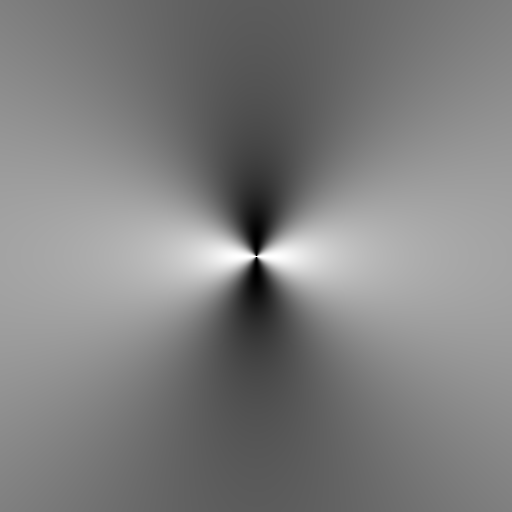
\includegraphics[scale=0.25]{figures/unified_dfilt_wr_sqrt8.png}
 }
 \hfill
 \subtop[$U_{10}=\sqrt{50}$]
 {
 
\includegraphics[scale=0.25]{figures/unified_dfilt_wr_sqrt50.png}
 }
 \hfill
 \subtop[$U_{10}=\sqrt{200}$]
 {
 
\includegraphics[scale=0.25]{figures/unified_dfilt_wr_sqrt200.png}
 }
 \subtop
 {
 
\includegraphics[scale=0.25]{figures/unified_dfilt_wur_sqrt2.png}
 }
 \hfill
 \subtop
 {
 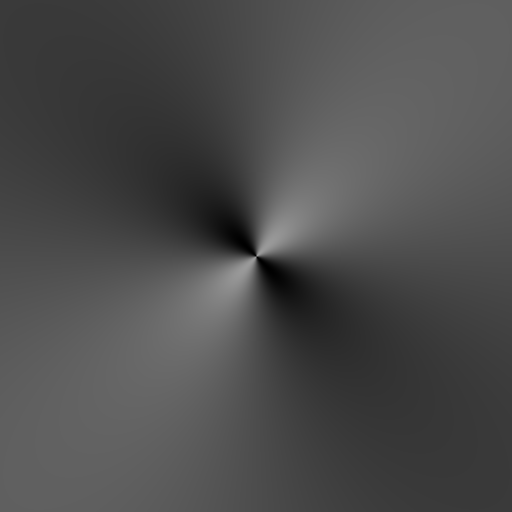
\includegraphics[scale=0.25]{figures/unified_dfilt_wur_sqrt8.png}
 }
 \hfill
 \subtop
 {
 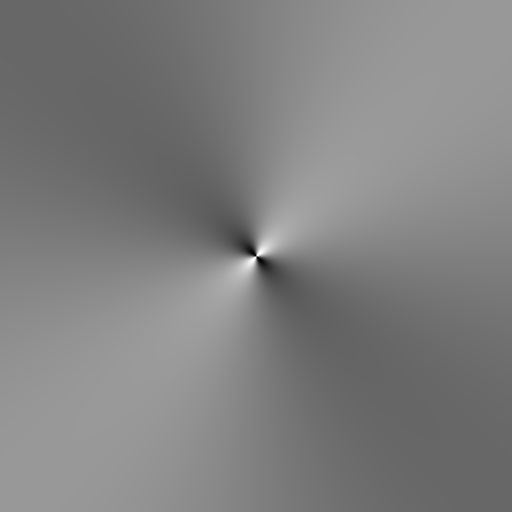
\includegraphics[scale=0.25]{figures/unified_dfilt_wur_sqrt50.png}
 }
 \hfill
 \subtop
 {
 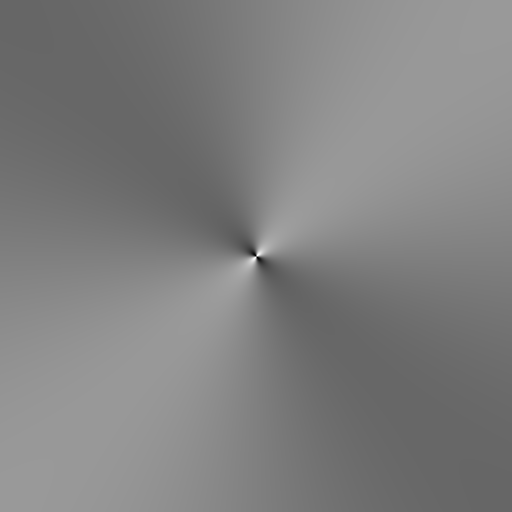
\includegraphics[scale=0.25]{figures/unified_dfilt_wur_sqrt200.png}
 }
\caption{A set of instances of the directional spreading function by
\citet{article:Elfouhaily1997}. Each column 
corresponds to a different wind speed, starting with the weakest one at the 
left. In the top row, the wind direction points to the right, in the bottom row 
to the upper right.}
\label{fig:unified_directional_filter}
\end{figure}
%

As one may see from Equation~\ref{eq:unified:theta}, the Unified spectrum's
directional spread is given as follows:
%
\begin{align}
D(k, \theta) &= \frac{1}{2\pi}\{1 + \Delta(k) + \cos[2(\theta - 
\theta_p)]\}
\end{align}
where $\theta_p$ is the direction of travel of the waves at the spectral peak.
The remaining terms are:
\begin{align*}
\Delta(k) = \tanh\left[a_0 + a_p\left(\frac{c}{c_p}\right)^{2.5} + 
a_m\left(\frac{c_m}{c}\right)^{2.5}\right]
\end{align*}
with
\begin{align*}
a_m = 0.13 \frac{u^{\ast}}{c_m} && a_0 = \frac{\log(2)}{4} && a_p = 4
\end{align*}
$c$ is the phase speed, $c_p$ is the phase speed at the spectral peak, and $c_m$
is the minimum phase speed at $k_m$. Moreover, $a_0$ and $a_p$ are constants,
whereas $a_m$ is a function for high-frequency waves dependent upon the friction
velocity $u^\ast$ and minimum phase speed $c_m$.
Figure~\ref{fig:unified_directional_filter} depicts example
instances of the Unified spectrum's directional spread. One can see that the
directional spread is~\emph{centrosymmetrical}, in short
$D(k, \theta) = D(k, \theta \pm \pi)$. As a consequence the two-dimensional
\wavenumber spectrum is centrosymmetrical, too. Therefore, the Unified spectrum
satisfies the following conditions:
\begin{align*}
\Theta(k, \theta) &= \Theta(k, \theta \pm \pi) & \Theta(\mvec{k}) &= \Theta(-\mvec{k})
\end{align*}
%
\subsection{Phillips Spectrum}
\label{sec:phillips_spectrum}
%
The Phillips Spectrum, as introduced by \cite{course:simulatingocean},
is an ad-hoc formulation of a two-dimensional \wavenumber spectrum $\Theta(\mvec{k})$.
It has been developed with computer graphic purposes in mind and is loosely
based on \citet{article:Phillips1958,article:Phillips1985}.
We may write \citeauthor{course:simulatingocean}'s
formulation of the Phillips Spectrum as follows:
%
\begin{equation}
\label{eq:phillips_spectrum}
 \Theta(\mvec{k}) = A\frac{\exp\left(-(kL)^{-2}-(kl)^2\right)}{k^4}\abs{\transpose{\mvec{k}_n}\mvec{w}_n}^2
\end{equation}
with
\begin{align*}
 \mvec{k}_n = \frac{\mvec{k}}{\norm{\mvec{k}}} = \frac{\mvec{k}}{k} && \mvec{w}_n = \frac{\mvec{w}}{\norm{\mvec{w}}}
\end{align*}
% where $A$ and $l$ are numeric constants to be chosen by the user. The numeric
% constant $A$ represents a scaling factor which we will discuss at a later point.
% The vector $\mvec{k}_n$ is the \wavevector $\mvec{k}$ at unit length:
% \begin{equation}
%  \mvec{k}_n = \frac{\mvec{k}}{\norm{\mvec{k}}} = \frac{\mvec{k}}{k}
% \end{equation}
% Similarly, $\mvec{w}_n$ is the wind vector $\mvec{w}$ at unit length:
% \begin{equation}
%  \mvec{w}_n = \frac{\mvec{w}}{\norm{\mvec{w}}}
% \end{equation}
% where $\mvec{w}$ encodes wind direction and wind speed $\norm{\mvec{w}}$.
% 
% 
% \mvec{k}_n = \frac{\mvec{k}}{\norm{\mvec{k}}} = \frac{\mvec{k}}{k}\\
% \mvec{w}_n = \frac{\mvec{w}}{\norm{\mvec{w}}}\\
% L = \frac{\norm{\mvec{w}}^2}{g}
% \end{gather}
%
where $A$ and $l$ are numeric constants, and $\mvec{w}$ encodes wind 
direction and wind speed $\norm{\mvec{w}}$. The numeric constant $A$ represents 
a scaling factor which we will discuss at a later point.  According to 
\citeauthor{course:simulatingocean}, $L$ defines the largest possible wave
arising from a continuous wind of speed $\norm{\mvec{w}}$. The parameter $l$ on 
the other hand acts as a frequency filter, it controls the suppression of energy
contributed by high \wavenumbers $k$. In order to accomplish that, it is
mandatory for $l$ to be several orders of magnitude smaller than $L$. The author
chose the following as a default value for $l$:
\begin{equation*}
 l = 10^{-3}L
\end{equation*}
Moreover, it follows from Equation~\ref{eq:phillips_spectrum} that setting 
${l = 0}$ disables any \wavenumber based suppression of energy. Additionally,
one may see that \citeauthor{course:simulatingocean} employs a one dimensional
\wavenumber spectrum, which is as follows:
\begin{equation}
\label{eq:phillips_wavenumber_spectrum}
  \Theta(k) = A\frac{\exp\left(-(kL)^{-2}-(kl)^2\right)}{k^4}
\end{equation}
% If we take a closer look at Equation~\ref{eq:phillips_spectrum} one may notice 
% similarities to a one dimensional frequency spectrum in combination with a 
% directional spread as seen in Equation~\ref{eq:directional_frequency_spectrum}. 
% We may separate the terms involved as follows:
% \begin{equation}
% \label{eq:phillips_spectrum_separated}
%  \Theta(\mvec{k}) = \underbrace{A}_{Scale}\underbrace{\frac{\exp\left(-(kL)^{-2}-(kl)^2\right)}{k^4}}_{\substack{one~dimensional\\wavenumber\\spectrum}}\underbrace{\abs{\transpose{\mvec{k}_n}\mvec{w}_n}^2}_{\substack{directional\\spread}}
% \end{equation}
%
\begin{figure}
\centering
\begin{tikzpicture}
\begin{groupplot}[
	group style={
		columns=2,
		xlabels at=edge bottom,
		ylabels at=edge left,
		group name=plots,
	},
    xlabel={\Wavenumber~$k$~(\si{\radian\per\second})},
    ylabel={Energy~$\Theta$~(\si{\cubic\meter\per\radian})},
%     legend columns=-1,
	width=0.5\textwidth,
	]
\nextgroupplot[
    legend style={draw=none},
    every axis legend/.append style={nodes={right}},
	xticklabel style={/pgf/number format/fixed},
	restrict x to domain=0:0.125,
	]
\addplot[
    color=red,
    solid,
	]
    table [col sep=comma]{figures/phillips_10_k.dat};
	\addlegendentry{\SI{10.0}{\meter\per\second}}
\addplot[
    color=green,
    solid,
	]
    table [col sep=comma]{figures/phillips_12_k.dat};
	\addlegendentry{\SI{12.5}{\meter\per\second}}
\addplot[
    color=magenta,
    solid,
	]
    table [col sep=comma]{figures/phillips_15_k.dat};
	\addlegendentry{\SI{15.0}{\meter\per\second}}
\addplot[
    color=black,
    solid,
	]
    table [col sep=comma]{figures/phillips_17_k.dat};
	\addlegendentry{\SI{17.5}{\meter\per\second}}
\addplot[
    color=blue,
    solid,
	]
    table [col sep=comma]{figures/phillips_20_k.dat};
	\addlegendentry{\SI{20.0}{\meter\per\second}}
\nextgroupplot[
    legend style={draw=none},
    every axis legend/.append style={nodes={right}},
	restrict x to domain=0:0.25,
]
\addplot[
    color=black,
    solid,
    ]
    table [col sep=comma]{figures/phillips_12_k_0_025.dat};
\addlegendentry{Phillips}
\addplot[
    color=blue,
    solid,
	]
    table [
		col sep=comma, 
		x expr=\thisrowno{0},
		y expr=\thisrowno{1}*1000,
	]
	{figures/pm_12_k.dat};
\addlegendentry{PM~$\times 10^3$}
\addplot[
    color=magenta,
    solid,
	]
    table [
		col sep=comma, 
		x expr=\thisrowno{0},
		y expr=\thisrowno{1}*1000,
	]
	{figures/j_12_200km_k.dat};
\addlegendentry{JONSWAP~$\times 10^3$}
\end{groupplot}
\end{tikzpicture}
\caption{Left: The one dimensional \wavenumber spectrum term of the Phillips 
frequency spectrum with different wind speed values $\norm{\mvec{w}}$. Right: 
The difference in scale between the Phillips spectrum and both, the Pierson 
Moskowitz spectrum and the JONSWAP spectrum, amounts to at least a factor of 
$10^3$ ($U_{10}=\norm{\mvec{w}}=\SI{12.5}{\meter\per\second}$, $F=\SI{200}{\km}$).
% The shape of the spectrum resembles the Pierson Moskowitz spectrum.
}
\label{fig:phillips_spectra}
\end{figure}
%
A set of instances of the one dimensional \wavenumber spectrum term are depicted 
in Figure~\ref{fig:phillips_spectra}. One may see that the shape of the 
spectrum is similar to the Pierson Moskowitz one in Figure~\ref{fig:pm_spectra}, 
with the frequency range of the spectrum peak being located at even lower 
frequencies than the Pierson Moskowitz and JONSWAP ones. The magnitude of the 
energy on the other hand exceeds the one given by Pierson Moskowitz and JONWAP 
by at least a factor of $10^3$. Recall that both the Pierson Moskowitz and the 
JONSWAP model are based on real world data aquired on the ocean, then we may 
reason that those models give us a value range for energy precise enough to 
generate believable results. Therefore we need to rescale the energy obtained 
from the Phillips spectrum into that range. It seemed reasonable to us
that that is the purpose of the numeric constant $A$ in 
Equations~\ref{eq:phillips_spectrum} and \ref{eq:phillips_wavenumber_spectrum}. 
Since \citeauthor{course:simulatingocean} does not give any information about
$A$, choosing a value that  scales energy appropriately for all reasonable
input parametrisations has proven to be difficult. The constant
$\alpha = 8.1 \times 10^{-3}$ as given by \citet{article:PiersonMoskowitz1964}
(Equation~\ref{eq:pierson_moskowitz_theta_old}) seemed to be promising
initially, in the end the author settled for the following more adaptive
solution:
\begin{align*}
 A = \frac{0.81}{LK}B && B \in \interval{0}{1}
\end{align*}
where $L$ and $K$ represent side lengths in meters of the rectangular area 
we want to synthesize.
%
\begin{figure}
 \centering
 \subbottom[$\cos^2$]
 {
 \label{subfig:directional_spread_cos2_r}
 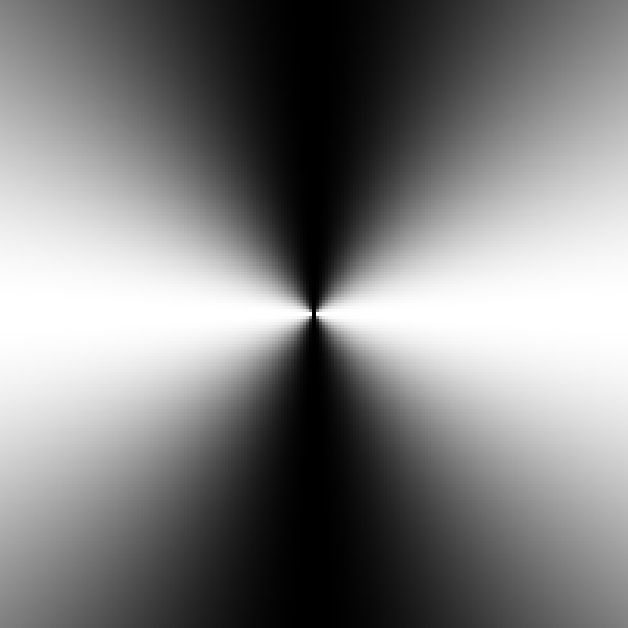
\includegraphics[scale=0.6]{figures/phillips_dir_r_exponent_2.png}
 }
 \hfill
 \subbottom[$\cos^4$]
 {
 \label{subfig:directional_spread_cos4_r}
 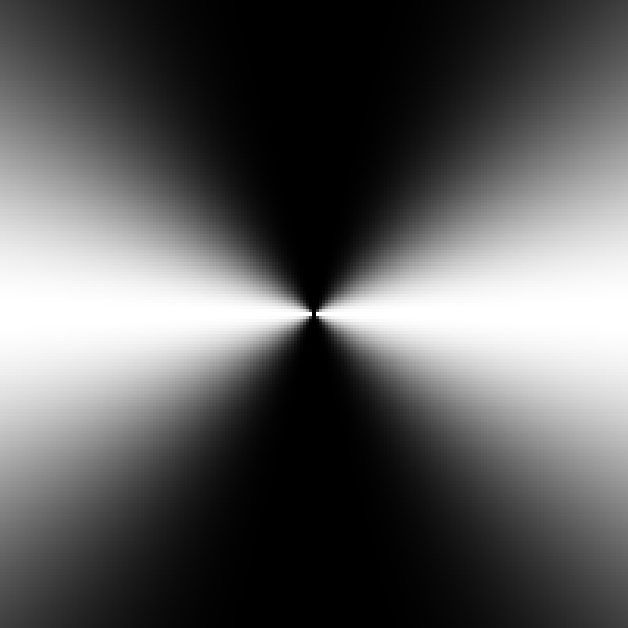
\includegraphics[scale=0.6]{figures/phillips_dir_r_exponent_4.png}
 }
 \hfill
 \subbottom[$\cos^2$]
 {
 \label{subfig:directional_spread_cos2_ur}
 
\includegraphics[scale=0.6]{figures/phillips_dir_ur_exponent_2.png}
 }
 \hfill
 \subbottom[$\cos^4$]
 {
 \label{subfig:directional_spread_cos4_ur}
 
\includegraphics[scale=0.6]{figures/phillips_dir_ur_exponent_4.png}
 }
\caption{Example instances of the Phillips directional spreading function with 
exponents $2$ and $4$. For~\subcaptionref{subfig:directional_spread_cos2_r} and
\subcaptionref{subfig:directional_spread_cos4_r} the wind direction poins to 
the right, for \subcaptionref{subfig:directional_spread_cos2_ur} and
\subcaptionref{subfig:directional_spread_cos4_ur} it points to the upper right. 
The directional spread with an exponent of $4$ is distinctly more narrow 
than the one with an exponent of $2$. Moreover, all instances are
centrosymmetrical.}
\label{fig:phillips_directional_term}
\end{figure}
%

Now that we have discussed the one dimensional \wavenumber spectrum and the 
scale factor $A$, we move on to the directional term from 
Equation~\ref{eq:phillips_spectrum}, which is as follows:
\begin{equation*}
 D(\mvec{k})~=~\abs{\transpose{\mvec{k}_n}\mvec{w}_n}^2~=~\abs{\cos(\theta)}^2
\end{equation*}
where $\theta$ is the angle between normalized \wavevector $\mvec{k}_n$ and
normalised wind direction $\mvec{w}_n$.
% The above is a simple cosinus 
% term raised to the power of two, with normalised \wavevector $\mvec{k}$ and 
% normalised wind vector $\mvec{w}$ as input.
We may increase the exponent in 
order to make the resulting directional spread more narrow. Moreover, as only
the  absolute value of the cosinus is taken into account, the result is
centrosymmetrical. Figure \ref{fig:phillips_directional_term} gives an
illustration of the directional spread with different wind directions and
different exponents.

Recall that the directional spread distributes the energy represented by
$\Theta(k)$ among all directions, without changing the amount of energy at
\wavenumber $k$. Energy is conserved, therefore we may write:
\begin{align*}
\int_{\theta=-\pi}^{\pi}D(k,\theta)~\mathrm{d}\theta = 1 && D(k,\theta) &\geq 0
\end{align*}
We insert two variants of the Phillips directional spread into the integral:
\begin{align*}
\int_{\theta=-\pi}^{\pi} \abs{\cos(\theta)}^2~\mathrm{d}\theta &= \pi \\
\int_{\theta=-\pi}^{\pi} \abs{\cos(\theta)}^4~\mathrm{d}\theta &= \frac{3\pi}{4}
\end{align*}
As one can see, the results are \emph{not} equal one, therefore energy is 
\emph{not} conserved. In combination with the unusual magnitude of energy 
output by the one dimensional Phillips \wavenumber spectrum, it is really 
difficult to find an appropriate scale factor $A$ in order to generate 
plausible ocean surfaces.
%
